\pdfoutput=1
\documentclass[11pt]{article}
% \usepackage[review]{acl}
\usepackage{acl}
\usepackage{times}
\usepackage{latexsym}
\usepackage{multirow}
\usepackage{sidecap}
\usepackage{amsthm}
\usepackage{amsmath}
\usepackage{amssymb}
\usepackage{amsfonts}
\usepackage{verbatim} % for multi-line comments
\usepackage{url}
\usepackage{pifont}
\usepackage{eqparbox}
\usepackage{arydshln} % for dashed line in tables 
\usepackage{bigstrut}
\usepackage{comment}
% \usepackage{minted}
\usepackage[linewidth=1pt]{mdframed}
\usepackage{framed}
\usepackage{xcolor,colortbl}
\usepackage{pgffor}
\usepackage{comment}
\usepackage{graphicx}
\usepackage{booktabs}
\usepackage{subcaption}
\usepackage{enumitem}
\usepackage{makecell}
% \usepackage{arydshln}
% \usepackage{tabularray}
\usepackage{boxedminipage}
\usepackage{xspace}
\usepackage{array}
\usepackage{framed}
\usepackage{caption}
\usepackage{subcaption}
\usepackage{framed}
% \usepackage{colortbl}
\usepackage{array}
\usepackage{listings}
\usepackage{adjustbox}
\usepackage{tikz}
\usetikzlibrary{tikzmark}
\usepackage{enumitem}
\usepackage{bigstrut}
% \usepackage{libertine}
\usepackage[notextcomp]{stix}

\renewcommand\theadalign{bc}
\renewcommand\theadfont{\bfseries}
\renewcommand\theadgape{\Gape[4pt]}
\renewcommand\cellgape{\Gape[4pt]}




\newcolumntype{L}[1]{>{\raggedright\let\newline\\\arraybackslash\hspace{0pt}}m{#1}}
\newcolumntype{C}[1]{>{\centering\let\newline\\\arraybackslash\hspace{0pt}}m{#1}}
\newcolumntype{R}[1]{>{\raggedleft\let\newline\\\arraybackslash\hspace{0pt}}m{#1}}

% For proper rendering and hyphenation of words containing Latin characters (including in bib files)
\usepackage[T1]{fontenc}
% For Vietnamese characters
% \usepackage[T5]{fontenc}
% See https://www.latex-project.org/help/documentation/encguide.pdf for other character sets

% This assumes your files are encoded as UTF8
\usepackage[utf8]{inputenc}

% This is not strictly necessary, and may be commented out,
% but it will improve the layout of the manuscript,
% and will typically save some space.
\usepackage{microtype}
\usepackage{soul}
% \usepackage{tgbonum}

% If the title and author information does not fit in the area allocated, uncomment the following
%
%\setlength\titlebox{<dim>}
%
% and set <dim> to something 5cm or larger.

\setlength\fboxsep{1pt}
\definecolor{lightergray}{RGB}{230,230,230}
\definecolor{DarkRed}{RGB}{130,25,0}
\definecolor{DarkGreen}{RGB}{30,130,30}
\definecolor{DarkBlue}{RGB}{0,0,250}
\definecolor{purple}{rgb}{0.5,0,1}
\definecolor{dcyan}{rgb}{0.2,0.6,0.5}
\definecolor{darkgreen}{rgb}{0,200,0}
\definecolor{light-gray}{gray}{0.95} % used in table
% \definecolor{darkgreen}{RGB}{0,140,0}
\definecolor{darkred}{RGB}{200,0,0}
\definecolor{lightgreen}{RGB}{231,255,219}
\definecolor{lightred}{RGB}{252,231,234}
\definecolor{lightyellow}{RGB}{250,253,191}
% \definecolor{DarkRed}{RGB}{130,25,0}


\newcommand{\redtext}[1]{\colorbox{lightred}{#1}\xspace}
\newcommand{\greentext}[1]{\colorbox{lightgreen}{#1}\xspace}
\newcommand{\yellowtext}[1]{\colorbox{lightyellow}{#1}\xspace}
\newcommand{\bluetext}[1]{\colorbox{lightblue}{#1}\xspace}


\newcommand{\cmark}{\textcolor{DarkGreen}{\ding{51}}}
\newcommand{\xmark}{\textcolor{red}{\ding{55}}}%
\newcommand{\todo}[1]{{\color{red} [TODO: {#1}]}}
\newcommand{\yizhong}[1]{\textcolor{violet}{[YZ: #1]}}
\newcommand{\yeganeh}[1]{\textcolor{magenta}{[YK: #1]}}
\newcommand{\swaroop}[1]{\textcolor{cyan}{[SM: #1]}}
\newcommand{\daniel}[1]{\textcolor{blue}{[DK: #1]}}
\newcommand{\hanna}[1]{\textcolor{brown}{[HH: #1]}}
\newcommand{\nascomment}[1]{\textcolor{blue}{\textbf{[#1 -- \textsc{nas}]}}}
\newcommand{\alisa}[1]{\textcolor{purple}{\textbf{[#1 -- \textsc{al}]}}}

% acronyms 
\newcommand{\name}{\textsc{Self-Instruct}}
\newcommand{\dataset}{\textsc{Diverse-Instructions}} % Free-instructions? LM-Instructions
\newcommand{\wildins}{\textsc{Wild-Instructions}}
\newcommand{\supernat}{\textsc{Super-NaturalInstructions}}
% \newcommand{\supernatShort}{\textsc{Sup-NatInst}}
\newcommand{\supernatShort}{\textsc{SuperNI}}
\newcommand{\tkinstruct}{\textsc{T$k$-Instruct}}
\newcommand{\tzero}{\textsc{T$0$}}
\newcommand{\natins}{\textsc{NaturalInstructions}}
\newcommand{\natinsShort}{\textsc{NatInst}}
\newcommand{\crossfit}{\textsc{CrossFit}}
\newcommand{\flan}{\textsc{FLAN}}
\newcommand{\gptthree}{\textsc{GPT3}}
\newcommand{\gptself}{\textsc{GPT3}$_{\textsc{Self-Inst}}$}
% \newcommand{\gptinstruct}[1]{\textsc{GPT3}$^{\text{Instruct}}_{\text{#1}}$}
\newcommand{\gptinstruct}[1]{$\text{InstructGPT}_{\text{#1}}$}
\newcommand{\zest}{\textsc{Zest}}
\newcommand{\promptsource}{\textsc{PromptSource}}
\newcommand{\bigbench}{\textsc{BigBench}}


% If the title and author information does not fit in the area allocated, uncomment the following
%
%\setlength\titlebox{<dim>}
%
% and set <dim> to something 5cm or larger.


\title{Language Model Self Instructing Enables Better Zero-shot Learners}
\title{Adjusting Language Models to Follow Instructions \\ with (Almost) No Human Annotations}
\title{Machine Self Instructing \\ Enables More Diverse Zero-shot Instruction Following}
\title{Language Model Self Instructing \\ Enables More Diverse Zero-shot Instruction Following}
\title{Language Model Self Instructing \\ Enables More Diverse Instruction Following Behaviors}
\title{\emph{Self-Instructing} Language Models to Align with Diverse Instruction}
\title{Self-Instructing Align Language Models with Diverse Commands}
\title{Self-Instructing Off-the-Shelf Language Models}
\title{Language Model Self-Instructing Enables Diverse Instruction Following}
\title{Adjusting Language Models to Follow Instructions \\ with Light Human Annotation}
\title{Adjusting Language Models to Follow Instructions \\ with Model Self-Instructing}
\title{Language Models are Self-Instructable}
\title{Language Models Self-Instructing}
\title{Language Models Can Self-Instruct}
\title{Self-Instructing Language Models}
\title{Language Models are Zero-shot Self-Instructors}
\title{Language Models Self Instruct}
\title{Self-Instruction of Language Models}
\title{\name{}: Adjusting Language Model to Follow \\ Instructions with its Own Generations}
\title{\name{}: Aligning Language Model \\ with Self Generated Instructions}

%\title{Self-Instruct: Learn to Follow Instructions by Self-creation of Instruction Tasks}
%\title{Self-Instruct: Learn from Instructions by Creating your Own Instruction Dataset}


% use a fancier font style for \tt 
\renewcommand\ttdefault{cmtt}

\author{
Yizhong Wang\textsuperscript{$\clubsuit$} \;\;\;  
Yeganeh Kordi\textsuperscript{$\diamondsuit$} \;\;\;
Swaroop Mishra\textsuperscript{$\heartsuit$} \;\;\; 
\textbf{Alisa Liu}\textsuperscript{$\clubsuit$}\\ 
\textbf{Noah A. Smith}\textsuperscript{$\clubsuit$}\textsuperscript{$+$} \;\;\;
\textbf{Daniel Khashabi}\textsuperscript{$\spadesuit$} \; \;\;
\textbf{Hannaneh Hajishirzi}\textsuperscript{$\clubsuit$}\textsuperscript{$+$}\\
  \textsuperscript{$\clubsuit$}University of Washington \; 
  \textsuperscript{$\diamondsuit$}Tehran Polytechnic \;
  \textsuperscript{$\heartsuit$}Arizona State University \\
  \textsuperscript{$\spadesuit$}Johns Hopkins University\; \textsuperscript{$+$}Allen Institute for AI \\
  {  \texttt{yizhongw@cs.washington.edu} } \\}

\begin{document}
\maketitle
\begin{abstract}


Large ``instruction-tuned'' language models (finetuned to respond to instructions) have demonstrated a remarkable ability to generalize zero-shot to new tasks. 
Nevertheless, they depend heavily on 
% ``instructions'' (natural language task definitions) 
human-written instruction data
% collected either from existing NLP datasets or 
that is limited in quantity, diversity, and creativity, therefore hindering the generality of the tuned model. 
% \swaroop{Humans have a remarkable ability to learn instruction-following from a few supervised instruction tasks, probably by bootstrapping}.
% Large language models have demonstrated the ability to conduct many tasks in a zero-shot manner by following instructions. Existing studies have shown that such instruction following behavior can be better induced by an instruction tuning stage, where a diverse set of training tasks are used to finetune the model to respond to instructions. However, these tasks and their instructions are either collected from existing NLP datasets or newly written by human annotators. This largely limits their quantity, diversity and creativity, hindering the generality of the tuned model. 
We introduce \name{}, a  framework for improving the instruction-following capabilities of pretrained language models by bootstrapping off its own generations. 
% We found that large pretrained language models are able to generate creative instructions as well as relatively high-quality input and output pairs when prompted with a small number of seed tasks.
Our pipeline generates instruction, input, and output samples from a language model, then prunes them before using them to finetune the original model.
% We test out its effectiveness with vanilla \gptthree{} as a case study, and generate over 50K instructions paired up with 80K instances. 
% To test out the effectiveness of \name, we experiment with vanilla \gptthree{} (not instruction-tuned). 
% This leads to  a large number of natural language instructions and corresponding instances (input-output pairs), which we then use to fine-tune \swaroop{instruction-tune} the \gptthree{} model itself. 
% This data is, in turn, used to finetune the \gptthree{} model itself.
% Evaluation on \supernat{} benchmark indicates that the resulting model \gptinstruct{{\color{blue}Self-Ins}}
% results in 33.1\% gain over \gptthree{}, on par with the performance of \gptinstruct{{\color{blue}OpenAI}}
% Evaluation on the \supernat{} benchmark shows that the self-instructed version of GPT3 (a.k.a. \gptself) 
% \hanna{does the model start with gpt and uses your data? or does it start with instructGPT and trained on your data; with this naming it seems that you self train instruct gpt and get performance close to instrutgpt-001}
% \daniel{
% It is the former: start with GPT3. 
% }
% can achieve 33\% absolute improvement over the vanilla GPT3 on the testing NLP tasks, on par with the performance of \gptinstruct{001}
Applying our method to vanilla \gptthree{}, we demonstrate a 33\% absolute improvement over the original model on \supernat{}, on par with the performance of \gptinstruct{001}\footnote{
\label{footnote:gpt:instruct}Unless otherwise specified, our comparisons are with the 
{\tt text-davinci-001} engine. 
We focus on this engine since it is the closest to our experimental setup: supervised fine-tuning with human demonstrations. 
The newer engines are more powerful, though they use more data (e.g., code completion or latest user queries) or algorithms (e.g., PPO) that are difficult to compare with. 
% \nascomment{this point might also need to be made in the experiment section, reader will forget about seeing it here} \alisa{I think this footnote would be better somewhere else, not in the abstract}
}, which is trained with private user data and human annotations.
For further evaluation, we curate a set of expert-written instructions for novel tasks, and show through human evaluation that tuning GPT3 with \name{} outperforms using existing public instruction datasets by a large margin, leaving only a 5\% absolute gap behind \gptinstruct{001}.
% \nascomment{, which is much more expensive?  signal that this would be very hard to beat}. 
\name{} provides an almost annotation-free method for aligning pretrained language models with instructions, and we release our large synthetic dataset to facilitate future studies on instruction tuning\footnote{Code and data will be available at \url{https://github.com/yizhongw/self-instruct}.}.
% with limited reliance on human annotations 
% We release this large synthetic dataset, our seed tasks, and the human evaluation dataset to facilitate future studies on instruction tuning.


\begin{comment}
In this paper, we introduce a \name{}, a  framework which uses a pretrained language model itself to generate a large number of language instructions 
and corresponding instances (input-output pairs). 
This model-generated data can be used to bootstrap the instruction tuning of the model and enables better instruction following after several generation and training iterations. We show that this \name{} framework is effective for several models at different sizes or with different architectures, and brings consistent improvement as it grows until the size of 100K.
For example, we are able to improve GPT3's performance on xxx by yyy, matching InstructGPT which is trained with private human-written data.\yizhong{briefly compare with GPT3 and InstructGPT}. We believe that this method provides an annotation-free step for improving a pretrained language model before it is used for downstream tasks, and the resulting data will be valuable for future study on instruction tuning.
\end{comment}
\end{abstract}

\section{Introduction}
\label{sec:intro}
The recent  NLP literature has witnessed a tremendous amount of activity in building models that can follow natural language instructions~\citep[i.a.]{mishra2022cross,wei2022finetuned,sanh2022multitask,wang2022benchmarking,ouyang2022training,chung2022scaling}.
These developments are powered by two key components: large pre-trained language models (LM) and human-written instruction data.
% ;~\citealp{devlin2019bert,raffel2020exploring, brown2020language, chowdhery2022palm} \alisa{not sure these citations are necessary, and hinders readability}
\promptsource{}~\citep{bach2022promptsource} and \supernat{}~\citep{wang2022benchmarking} are two notable recent datasets that use extensive manual annotation for collecting instructions to construct \tzero~\cite{bach2022promptsource,sanh2022multitask} and \tkinstruct~\cite{wang2022benchmarking}. 
% \alisa{I think this previous sentence can be omitted} 
However, this process is costly and often suffers limited diversity given that most human generations tend to be popular NLP tasks, falling short of covering a true variety of tasks and different ways to describe them. 
Given these limitations, continuing to improve the quality of instruction-tuned  models 
% \nascomment{this is way too strong:} 
necessitates the development of alternative approaches for supervising instruction-tuned models. 
% \swaroop{comment-the motivation sounds like we will see a unsupervised learning approach in the next paragraph. How about adding the following to glue?}\swaroop{Evidently, Humans are capable of generalizing to unseen instructions with just a handful of supervised instructions. They could potentially be bootstraping the few supervision instances to create a large set of instances which can potentially help in simulation of various instruction-following scenarios}. \yizhong{Making analogy to human is risky, and I like the current motivation that human-annotated data is problematic. Let's keep the current version.}

% \daniel{
% I think the idea addresses two issues: 
% (1) cost of manual annotations 
% (2) lack of diversity in human annnotations. 
% Currently the text mentions (1) but does not cover (2)
% }


% \begin{figure}[t]
%     \centering
%     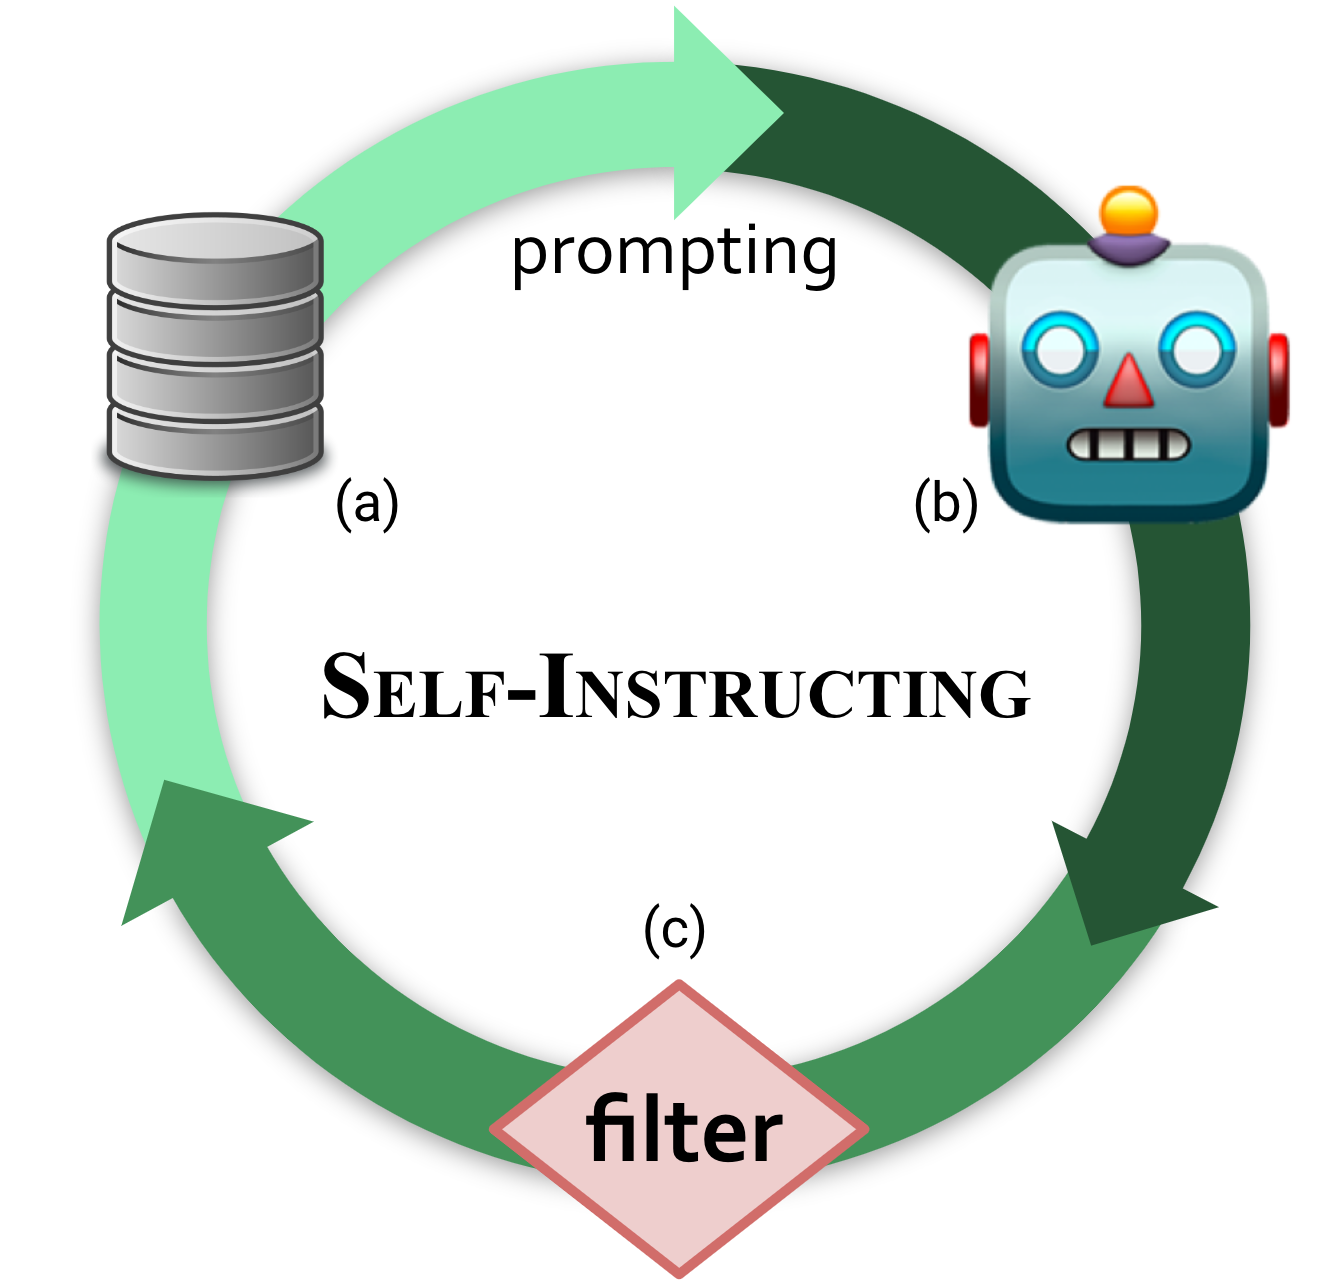
\includegraphics[scale=0.25, trim=0cm 0cm 0cm 0cm]{figures/teaser-1.png}
%     % figure here if you wanna modify it: https://docs.google.com/presentation/d/1GEYzNofuB_nCjhfFa2imfiye1rp3dgbeN6ALjXz2O2s/edit?usp=sharing 
%     \caption{
%         A high-level overview of \name{}. 
%          The process starts with a small seed set of instructions and their outputs (a). 
%          This seed set is then used to prompt an off-the-shelf LM to generate more language instructions/outputs (b), 
%          followed by filtering low-quality or repeated generations, and then added back to the initial repository of instructions. 
%          This bootstrapping cycle continues until there is little yield in each new cycle. 
%     }
%     \label{fig:teaster}
% \end{figure}

\begin{figure*}[ht]
    \centering
    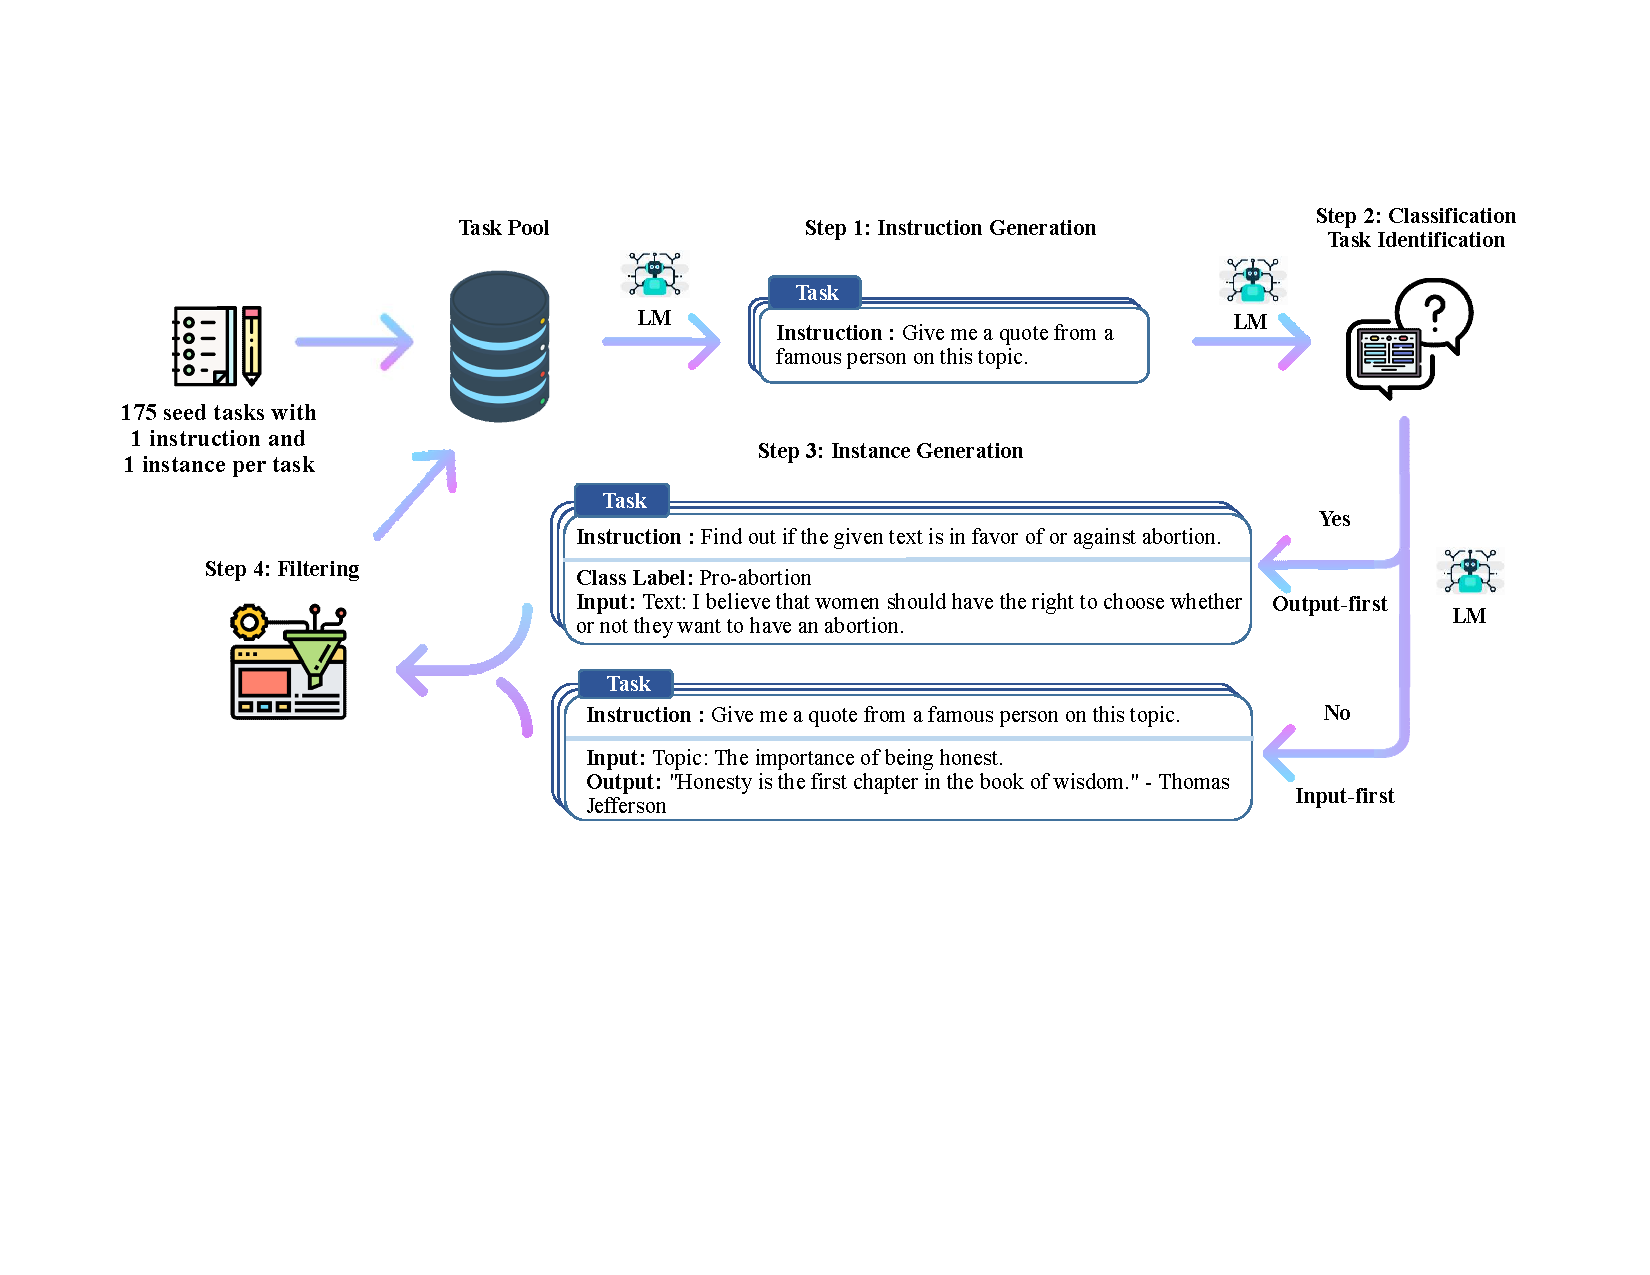
\includegraphics[width=\textwidth]{figures/data_generation_pipeline_v5.pdf}
    \caption{
     A high-level overview of \name{}. 
     The process starts with a small seed set of tasks (one instruction and one input-output instance for each task) as the task pool. 
     Random tasks are sampled from the task pool, and used to prompt an off-the-shelf LM to generate both new instructions and corresponding instances, 
     followed by filtering low-quality or similar generations, and then added back to the initial repository of tasks. The resulting data can be used for the instruction tuning of the language model itself later to follow instructions better. Tasks shown in the figure are generated by \gptthree{}. See \autoref{tab:generated_tasks} for more creative examples.
     %\daniel{the generated tasks don’t seem to be that innovative/creative/diverse (they look like typical NLP task) — which goes against what we’re saying about the diversification of tasks. %\nascomment{what is the little robot icon?  I don't understand; label it}}
    % Overview of the pipeline of using a language model to generate instruction data (instruction-input-output triples) and the resulting data is used for instruction tuning of the language model itself. 
    % Texts highlighted in green are generated by GPT3 language model (``davinci'' engine).
    }
    \label{fig:pipeline}
\end{figure*}

In this work, we introduce \name, a semi-automated process for instruction-tuning a pretrained LM using instructional signals from the model itself. 
% for extracting instructional signals from language models, which can subsequently be used to turning them into strong instruction-followers (see Fig.\ref{fig:teaster}). 
The overall process is an iterative bootstrapping algorithm (see \autoref{fig:pipeline}), which starts off with a limited (e.g., 175 in our study) seed set of manually-written instructions that are used to guide the overall generation. 
In the first phase, the model is prompted to generate instructions for new tasks. 
This step leverages the existing collection of instructions to create 
% more diverse \nascomment{I don't think our experiments demonstrate that the instructions are more diverse, tone this down} 
more broad-coverage instructions that define (often new) tasks.
Given the newly-generated set of instructions, the framework also creates input-output instances for them, which can be later used for supervising the instruction tuning. 
% model\todo{carefully define what these are and why they're needed.}.
Finally, various measures are used to prune low-quality and repeated instructions, before adding them to the task pool. 
This process can be repeated for many interactions until reaching a large number of tasks.
% the new additions are negligibly different. 
% \todo{it would be good to incorporate examples in the above paragraph}


To evaluate \name{} empirically, we run this framework on \gptthree{}~\cite{brown2020gpt3}, which is a vanilla LM (\S\ref{sec:generatd-data}).
The iterative \name{} process on this model leads to about 52k instructions, paired with about 82K instance inputs and target outputs. 
We observe that the resulting data provides a diverse range of creative tasks and over 50\% of them have less than 0.3 ROUGE-L overlaps with the seed instructions (\S\ref{subsec:diversity}).
On this resulting data, we build \gptself{} by fine-tuning \gptthree{} (i.e., the same model used for generating the instructional data). 
We evaluate \gptself{} in comparison to various other models on both typical NLP tasks included in \supernat{}~\cite{wang2022benchmarking}, and a set of new instructions that are created for novel usage of instruction-following models (\S\ref{sec:superni_results}). 
The \supernatShort{} results indicate that 
\gptself{} outperforms \gptthree{} (the original model) by a large margin (+33.1\%) and nearly matches the performance of \gptinstruct{001}. Moreover, our human evaluation on the newly-created instruction set shows that \gptself{} demonstrates a broad range of instruction following ability, outperforming models trained on other publicly available instruction datasets and leaving only a 5\% gap behind \gptinstruct{001}. 
% \todo{mention wild instructions}
% \yeganeh{An analysis of the performance of the \gptself{} on newly developed user-oriented instruction set demonstrates 44\% improvement over \gptthree{} and it's only 5\% less effective than \gptinstruct{001}}

% \todo{para on experimental findings: 
%  - built a model based on GPT3 
%  - the result beats GPT3 on NatIns 
%  - it is on-par with GPT3instruct 
%  - human evaluation
% }


In summary, our contributions are: (1) \name, a method for inducing instruction-following capability 
% for improving \swaroop{the instruction following capability of} 
with minimal human-labeled data;
(2) We demonstrate its effectiveness via extensive instruction-tuning experiments; 
% We conduct extensive experiments to demonstrate that instruction-tuning can keep benefiting from very diverse \nascomment{?} instructions. \swaroop{comment- this point looks weak, since the finding here is not new.} \alisa{agree, perhaps just say ``demonstrate its effectiveness''?}
% (3) We release two by-product datasets: (a) \dataset{} a large dataset of X \yeganeh{52K}\nascomment{don't forget to fill this in}  natural language tasks and instructions resulting from \name{} with \gptthree{} and  \ins{} \nascomment{broken command here}, (b) a collection of manually written tasks about daily activities. 
(3) We release a large synthetic dataset of 52K instructions and a set of manually-written novel tasks for building and evaluating future instruction-following models.




\section{Related Work}
\label{sec:related}

% \daniel{
% % 
% % prompt/instruction generation: all these works generate instructions given a few examples.. The space of tasks is pre-defined and fixed (i.e., they don’t bootstrap new tasks; but we do).
% % \cite{zhou2022large}
% % \cite{ye2022guess}
% % \cite{singh2022explaining}
% % \cite{gu2022learning}
% % \cite{honovich2022instruction}

% Incorporate this: 
% % Self-x: all these works use LMs to bootstrtap interesting inferences (meta-relevant to the purpose of this work). Also relevant to the "Self-training" paragrapg but not quite. So either want to broaden the "self-training" paragrapg to fit these in, or create a new paragraph. 
% \cite{zhao2022pre}
% \cite{zelikman2022star}
% \cite{welleck2022generating}
% \cite{zhou2022prompt}
% }
% \cite{}

\paragraph{Instruction-following language models.}
A series of works have found evidence that vanilla language models can be effective at following general language instructions if tuned with annotated ``instructional'' data -- datasets containing language instructional commands and their desired outcome based on human judgement~\cite{weller2020learning, mishra2022cross,wang2022benchmarking,wei2022finetuned,sanh2022multitask,ouyang2022training,parmar-etal-2022-boxbart, scialom2022continual, chung2022scaling,luo2022biotabqa,puri2022how,yin2022contintin,chakrabarty2022help,lin2022unsupervised,gupta2022improving,muennighoff2022crosslingual}. 
Additionally, they show a direct correlation between the size and diversity of the ``instructional'' data and the generalizability of resulting models to unseen tasks. 
Since these developments depend on human annotated ``instructional'' data, this poses a bottleneck for progress toward more generalizable models 
\cite[for example see Fig.~5a in][]{wang2022benchmarking}. 
Our work aims to tackle this bottleneck by reducing the dependence on human annotators. 

Additionally, despite the remarkable performance of models like  \gptinstruct{}~\cite{ouyang2022training}, their construction process remains quite opaque. 
% While there is some understanding of their construction (human annotation in model training loop), given its inaccessibility to the broader research community there is limited understanding about the source(s) of success. 
% Setting the difficulty of re-training gigantic models, 
In particular, the role of \emph{data} has remained understudied due to limited transparency and data released by major corporate entities behind these key models. 
% \nascomment{this sentence is repetitive and needs to be trimmed down to essentials:} 
Addressing such challenges necessitates the creation of a large-scale, public dataset covering a broad range of tasks.


% In particular, the role of supervised data has remained understudied due to limited data released by major corporate entities behind major models. In addition,  it is nearly impossible for the research community to extend  and re-train these  gigantic models. Addressing these two challenges necessitates the availability of large-scale public benchmarks of a broad range of NLP tasks and their instructions to facilitate developing and evaluating models that can generalize to unseen tasks.
% \cite{chung2022scaling}\\
    
Instruction-following models have also been of interest in the multi-modal learning literature \cite{fried2018speaker, shridhar2020alfred, min2022film, weir2022one}.
\name{}, as a general approach to expanding data, can potentially also be helpful in those settings; however, this is out of the scope of this work.

    
% TODO: cite some speaker following work.
% \cite{fried2018speaker}
% \cite{shridhar2020alfred}
% \daniel{Is this the message here? 
% Highlight that there is a literature of building instruction-following models in multi-modal or in embodied environments. 
% }

\paragraph{Language models for data generation and augmentation.}
A variety of works have relied on generative LMs for data generation~\cite{schick2021generating,wang2021towards,liu2022wanli,meng2022tuning} or augmentation~\cite{feng2021survey,yang2020generative,mekala2022intermediate}.  For example, \citet{schick2021generating} propose to replace human annotations \emph{of a given task} with prompting large LMs and use the resulting data for fine-tuning (often smaller) models in the context of SuperGLUE tasks~\cite{wang2019superglue}. 
While our work can be viewed as a form of ``augmentation,'' our work differs from this line in that it is \emph{not} specific to a particular task (say, QA or NLI). In contrast, a distinct motivation for \name{} is to bootstrap new task definitions that may not have been defined before by any NLP practitioner (though potentially still important for downstream users).  
% Put differently, within the \nascomment{I don't understand what you mean by guardrails} guardrails for our meta-task (responding to instructions), we prompt LMs to improvise diverse \nascomment{?} and creative instructions. 


    
    % \item An \href{https://openreview.net/forum?id=NiEtU7blzN}{ICLR 2023 submission} on model self improving.
    


\paragraph{Self-training.}
A typical self-training framework ~\cite{he2019revisiting, xie2020self, du2021self, amini2022self, huang2022large} uses trained models to assign labels to unlabeled data and then leverages the newly labeled data to improve the model. In a similar line, \citet {zhou2022prompt} use multiple prompts to specify a single task and propose
to regularize via prompt consistency, encouraging
consistent predictions over the
prompts. This allows either 
finetuning the model  with extra unlabeled
training data, or direct application at inference time.
While \name{} has some similarities with the self-training literature, most self-training methods assume a specific \textit{target task} as well as \textit{unlabeled examples} under it; in contrast, \name{} produces a variety of tasks from scratch.
% there are two key differences: (1) most self-training methods assume the existence of unlabeled examples and focus on assigning labels, and (2) assume a specific target task.
% Unlike most self-training methods, \name{} does not assume any specific target task and instead generates several varieties of tasks from scratch. 
% Nonetheless, self-training methods, such as the self-consistency~\cite{wang2022self} used by \citet{huang2022large} can be leveraged \nascomment{vague -- do we do it or not?  don't say what could be done without being clear whether we do it} in the final step of \name{} to improve the filtering method and subsequently the quality of instruction task collection.



% \name{} leverages pretrained models to build datasets (with instructions) almost from scratch, in contrast to most self-training methods that requires unlabeled examples. (2) \name{} is a task-agnostic method intended to build general-purpose models, in contrast to the most self-training methods that focuses on a model for some specific tasks.

% 1) they focus more on the output part with the assumption that unlabeled examples are available; while we need to generate both input and output fields as well as the instruction; 2) we don’t assume the target task, we need to generate many task from scratch

    % \cite{huang2022large}
    % \cite{amini2022self}
    % \cite{xie2020self}
    % \cite{he2019revisiting}
    % Key differences: 1. we focus on general-purpose models; 2. the initial model is a language model instead of a model built for specific tasks; 3. we use the model to generate instructions, input and output, build datasets from almost scratch. Most self-training methods focus on unlabeled examples but the inputs are given; 4. Self-training can actually be used in our final step to improve the data quality. Leave for future work.


\paragraph{Knowledge distillation.}
Knowledge distillation~\cite{hinton2015distilling,Sanh2019DistilBERTAD, west2021symbolic,luciecharlotte2022teachingsmallmodels} often involves the transfer of knowledge from larger models to smaller ones. \name{} can also be viewed as a form of ``knowledge distillation", however, it differs from this line in the following ways: (1) the source and target of distillation are the same, i.e., a model's knowledge is distilled to itself; (2) the content of distillation is in the form of an instruction task (i.e., instructions that define a task, and a set of examples that instantiate it).

\paragraph{Bootstrapping with limited resources.} A series of recent works use language models to bootstrap some inferences using specialized methods.  
% NPPrompt~\cite{zhao2022pre} uses a model's own embeddings to automatically find relevant words \nascomment{confused here, not sure what you mean} to labels and this way reduces the dependency on verbalizers \nascomment{what are verbalizers?}.
NPPrompt~\cite{zhao2022pre} provides a method to generate predictions for semantic labels without any fine-tuning. It uses a model's own embeddings to automatically find words relevant to the label of the data sample and hence reduces the dependency on manual mapping from model prediction to label (verbalizers).
% relevant words \nascomment{confused here, not sure what you mean} to labels and this way reduces the dependency on verbalizers \nascomment{what are verbalizers?}.
STAR~\cite{zelikman2022star} iteratively leverages a small number of rationale examples and a large dataset without rationales, to bootstrap a model's ability to perform reasoning.  Self-Correction~\cite{welleck2022generating} decouples an imperfect base generator (model) from a separate corrector that learns to iteratively correct imperfect generations and demonstrates improvement over the base generator. Our work instead focuses on bootstrapping new tasks in the instruction paradigm.

\paragraph{Instruction generation.}
A series of recent works~\cite{zhou2022large, ye2022guess, singh2022explaining, honovich2022instruction} generate instructions of a task given a few examples. While \name{} also involves instruction generation, a major difference in our case is it is task-agnostic; we generate new tasks (instructions along with instances) from scratch.


% \daniel{
% 
% prompt/instruction generation: all these works generate instructions given a few examples.. The space of tasks is pre-defined and fixed (i.e., they don’t bootstrap new tasks; but we do).

% \cite{singh2022explaining}
% \cite{gu2022learning}
% \cite{honovich2022instruction}

% Incorporate this: 
% Self-x: all these works use LMs to bootstrtap interesting inferences (meta-relevant to the purpose of this work). Also relevant to the "Self-training" paragrapg but not quite. So either want to broaden the "self-training" paragrapg to fit these in, or create a new paragraph. 
% \cite{zhao2022pre}
% \cite{zelikman2022star}
% \cite{welleck2022generating}
% \cite{zhou2022prompt}
% }
% \cite{}



% Language models have been leveraged in the literature~\cite{petroni2019language, jiang2020can, burns2022discovering} to distill knowledge~\cite{cho2019efficacy, gou2021knowledge}; this knowledge is often used to assist models in downstream tasks.





% Language models have been leveraged in the literature~\cite{petroni2019language, jiang2020can, burns2022discovering} to distill knowledge~\cite{cho2019efficacy, gou2021knowledge}; this knowledge is often used to assist models in downstream tasks. 

% Our framework \name{} instead is focused on distilling knowledge in the form of instruction tasks (i.e. instructions that define a task, and a set of examples that instantiates it) which can potentially help develop a general-purpose model for a broad range of tasks.
% \daniel{
% This paragraph needs to be improved. My understanding is that "distillation" is often studied in the context of transferring knowledge e.g., (next-word probs in distilled-bert paper and many others) or (common-sense knowledge; symbolic knowledge distillation paper) from larger models to smaller ones.
% So there are two differences: 
% (1) The *source/target* of distillation: What we're doing is also a form of distillation, alas from a model to *itself*. 
% (2) The *content( of distillation: we're distilling "instructional" knowledge 
% }


% Model and knowledge Distillation
%     symbolic knowledge distillation 

% \daniel{
% if we want to argue that LMs already know and we just need a way to surface them: 
% \cite{burns2022discovering}
% Some of the arguments from the intro might also be useful here. 
% }



% \section{Language Model \name{}}
\section{Method}
\label{sec:method}

Annotating large-scale instruction data can be challenging for humans because it requires 1) creativity to come up with novel tasks and 2) expertise for writing the labeled instances for each task.
In this section, we detail our process for \name, which refers to the pipeline of generating tasks with a \textbf{vanilla pretrained language model} itself and then conducting instruction tuning with this generated data in order to align the language model to follow instructions better. This pipeline is depicted in \autoref{fig:pipeline}. 
% \yizhong{We should emphasize we use the vanilla language model.}

\subsection{Defining Instruction Data}
\label{subsec:instruction-data-definition}

The instruction data we want to generate contains a set of instructions $\{I_t\}$, each of which defines a task $t$ in natural language. Each task has one or more input-output instances $(X_t, Y_t)$.
A model $M$ is expected to produce the output $y$, given the task instruction $I_t$ and the instance input $x$: $M(I_t, x) = y, \;  \mbox{for} \ (x,y)\in (X_t, Y_t)$.
% For every instance, the model is expected to take the task instruction ${I_t}$ and the instance input $x$, and generate the output $y$. 
% Note that many instructions may not require additional input (e.g., ``write a poem'' itself is a valid request that models should respond to). In such cases, the instance input $x$ can be empty. 
Note that the instruction and instance input does not have a strict boundary in many cases. For example, ``write an essay about school safety'' can be a valid instruction that we expect models to respond to directly, while it can also be formulated as ``write an essay about the following topic'' as the instruction, and ``school safety'' as an instance input. To encourage the diversity of the data format, we allow such instructions that do not require additional input (i.e., $x$ is empty).

% \daniel{Somewhere (here?) we need to clarify how "input" and "instruction" are related or different, given that both are *inputs* to the model.} \yizhong{Check the updated version?}

\subsection{Automatic Instruction Data Generation}
\label{subsec:data-generation}

Our pipeline for generating the instruction data consists of four steps: 1) instruction generation, 2) identifying whether the instruction represents a classification task or not, 3) instance generation with the input-first or the output-first approach, and 4) filtering low-quality data.

\paragraph{Instruction Generation.}
\name{} is based on a finding that large pretrained language models can be prompted to generate new and novel instructions when presented with some existing instructions in the context. This provides us with a way to grow the instruction data from a small set of seed human-written instructions. 
We propose to generate a diverse set of instructions in a bootstrapping fashion. We initiate the task pool with 175 tasks (1 instruction and 1 instance for each task) written by our authors. For every step, we sample 8 task instructions from this pool as in-context examples.
% and use them as the prompt to make language models continue the generation of new instructions. 
Of the 8 instructions, 6 are from the human-written tasks,
 % to guarantee \nascomment{this is too strong, you have no guarantee} the quality
and 2 are from the model-generated tasks in previous steps to promote diversity. 
The prompting template is shown in \autoref{tab:instruction_generation_template}.
% provides the template for combining these instructions as a prompt to the language model. 
% We will show later that language models can successfully generate meaningful and creative instructions when prompted in this way.

\paragraph{Classification Task Identification.}
Because we need two different approaches for classification and non-classification tasks, we next identify whether the generated instruction represents a classification task or not.\footnote{More concretely, we regard tasks that have a limited and small output label space as classification tasks.} 
% 25 out of our 175 seed instructions are classification tasks. We mixed 12 classification seed instructions and 19 non-classification seed instructions as the prompt to ask the language model whether a newly generated instruction is  classification or not. 
We prompt vanilla GPT3 few-shot to determine this, using 12 classification instructions and 19 non-classification instructions from the seed tasks. The prompting template is shown in \autoref{tab:classification_task_identification_template}. 
% \autoref{tab:classification_task_identification_template} presents our prompt template for this step.

\paragraph{Instance Generation.}
Given the instructions and their task type, we generate instances for each instruction independently. This is challenging because it requires the model to understand what the target task is, based on the instruction, figure out what additional input fields are needed and generate them, and finally complete the task by producing the output. We found that pretrained language models can achieve this to a large extent when prompted with instruction-input-output in-context examples from other tasks.
% \alisa{confused about this sentence}
% Generating multiple instances is important for the model to learn to not only reply to the instructions, but also look at the input and learn to do reasoning over the input. See \ref{sec:prompting_templates} for the prompting templates.
A natural way to do this is the \textbf{Input-first Approach}, where we can ask a language model to come up with the input fields first based on the instruction, and then produce the corresponding output. This generation order is similar to how models are used to respond to instruction and input, but here with in-context examples from other tasks. The prompting template is shown in \autoref{tab:input-first-generation-template}. 

However, we found that this approach can generate inputs biased toward one label, especially for classification tasks (e.g., for grammar error detection, it usually generates grammatical input). Therefore, we additionally propose an
\textbf{Output-first Approach} for classification tasks, where we first generate the possible class labels, and then condition the input generation on each class label. The prompting template is shown in \autoref{tab:output-first-generation-template}.\footnote{In this work, we use a fixed set of seed tasks for prompting the instance generation, and thus only generate a small number of instances per task in one round. Future work can use randomly sampled tasks to prompt the model to generate a larger number of instances in multiple rounds.} We apply the output-first approach to the classification tasks identified in the former step, and the input-first approach to the remaining non-classification tasks.

% \daniel{
% Incorporate Yizhong's response: 
% The rationale of doing output-first is, for classification tasks, when generating the output first, we can easily generate all the possible class labels, and then condition the input generation on the class label. If using input first approach, the model's generation is usually biased to one label.
% }

\paragraph{Filtering and Postprocessing.}
\label{subsec:filtering}
To encourage diversity, a new instruction is added to the task pool only when its ROUGE-L overlap with any existing instruction is less than 0.7. 
We also exclude instructions that contain some specific keywords (e.g., images, pictures, graphs) that usually can not be processed by language models. When generating new instances for each instruction, we filter out instances that are exactly the same or those with the same input but different outputs.  


% \subsection{Self Training Algorithm}
% \label{subsec:self-training}

% The original GPT3 model usually cannot generate instances very well, especially for the challenging ones. We can use the self-training algorithm in \url{https://openreview.net/forum?id=SJgdnAVKDH} to bootstrap the model by doing the instance generation and instruction tuning alternatively in multiple rounds.

\subsection{Finetuning the LM to Follow Instructions}
\label{subsec:instruction-tuning}
After the creation of the large-scale instruction data, we use this data to finetune the original language model (i.e., \name{}). To do this, we concatenate the instruction and instance input as a prompt and train the model to generate the instance output in a standard supervised way. To make the model robust to different formats, we use multiple templates to encode the instruction and instance input together. For example, the instruction can be prefixed with ``Task:'' or not, the input can be prefixed with ``Input:'' or not, ``Output:'' can be appended at the end of the prompt, and different numbers of break lines can be put in the middle, etc.
% \nascomment{this is kind of vague.  what do we actually do?}


% \begin{figure*}[ht]
%   \adjustbox{valign=t}{
%   \begin{minipage}{0.55\linewidth}
%   \begin{subfigure}{\linewidth}
%     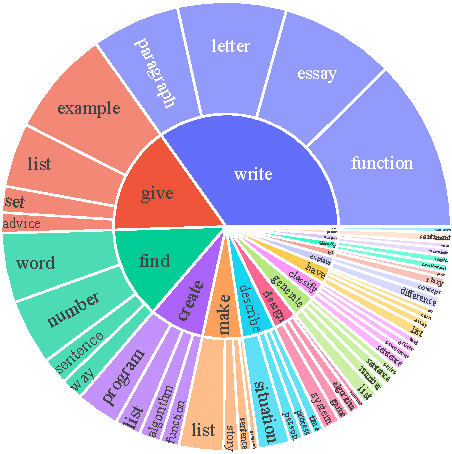
\includegraphics[width=\linewidth]{figures/instruction_sunburst_v2.pdf}
%     \caption{The top-20 most common root verbs (inner circle) and their top-4 direct noun objects (outer circle) in the generated instructions. Despite their diversity, the instructions shown here only account for 14\% of all the generated instructions because many instructions (e.g., ``Classify whether the user is satisfied with the service.'') do not contain such a verb-noun structure.}
%     \label{subfig:key-a}
%   \end{subfigure}\hfill
%   \end{minipage}
%   }
%   \hfill
%   \adjustbox{valign=t}{
%   \begin{minipage}{0.41\linewidth}
%     \vspace{10pt}
%     % \begin{subfigure}{0.475\linewidth}
%     %   \includegraphics[width=\linewidth]{figures/instruction_sunburst.pdf}
%     %   \caption{}\label{subfig:key-b}
%     % \end{subfigure}\hfill
%     \begin{subfigure}{0.95\linewidth}
%       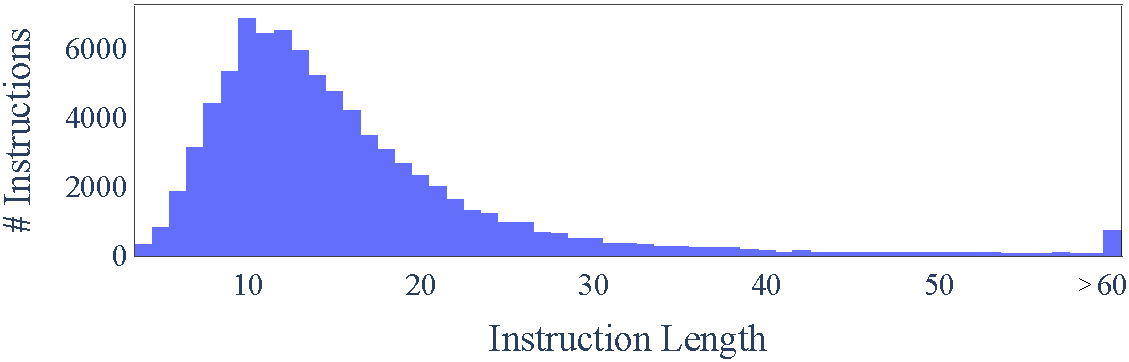
\includegraphics[width=\linewidth]{figures/instruction_length.pdf}
%       \caption{Distribution of instruction length (words)}\label{subfig:key-c}
%     \end{subfigure}
%     \medskip
%     \begin{subfigure}{0.95\linewidth}
%       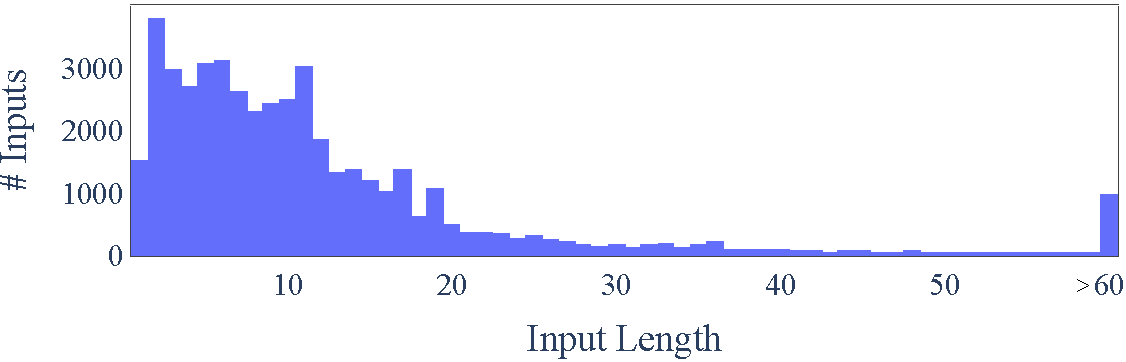
\includegraphics[width=\linewidth]{figures/input_length.pdf}
%       \caption{Distribution of non-empty input length (words)}\label{subfig:key-d}
%     \end{subfigure}\hfill
%     \begin{subfigure}{0.95\linewidth}
%       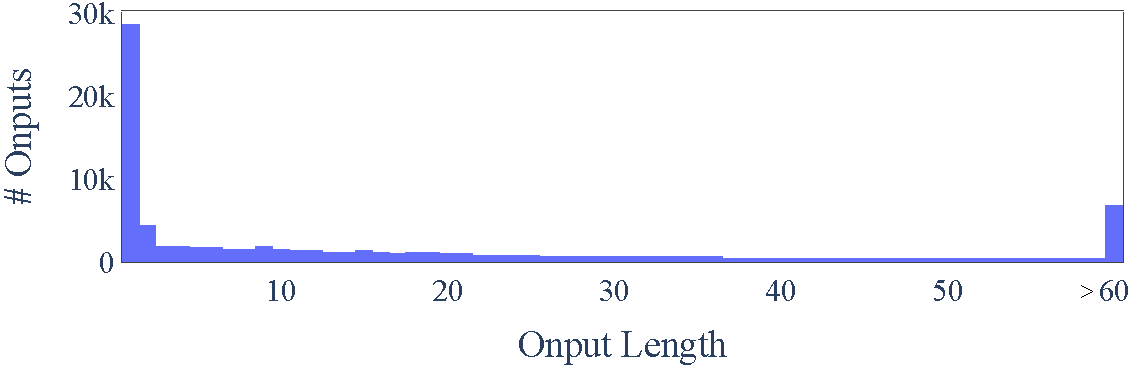
\includegraphics[width=\linewidth]{figures/output_length.pdf}
%       \caption{Distribution of output length (words)}\label{subfig:key-e}
%     \end{subfigure}\hfill
%   \end{minipage}
%   }
%   \caption{Distribution statistics of the generated instruction data. \todo{Make the font bigger. Make them different figures. Include a figure for the distance between generated instructions and their most similar seed tasks.}
%   % \daniel{state the unit of measurement (``token''?)} 
%   }
%   \label{fig:generated_data_distribution}
% \end{figure*}



\begin{figure*}[ht]
  \adjustbox{valign=t}{
  \begin{minipage}{0.55\linewidth}
    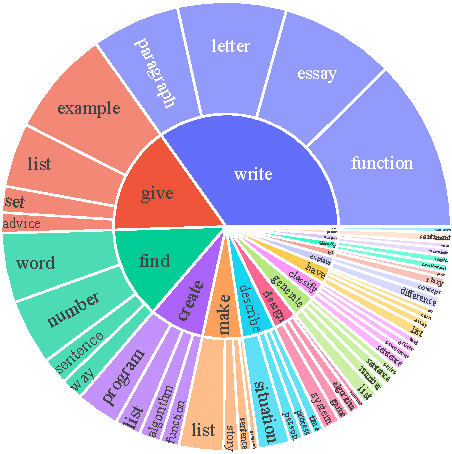
\includegraphics[width=0.98\linewidth,trim=0.5cm 0cm 0.35cm 0cm]{figures/instruction_sunburst_v2.pdf}
    \caption{The top 20 most common root verbs (inner circle) and their top 4 direct noun objects (outer circle) in the generated instructions. Despite their diversity, the instructions shown here only account for 14\% of all the generated instructions because many instructions (e.g., ``Classify whether the user is satisfied with the service.'') do not contain such a verb-noun structure. \label{fig:verb-noun-distribution}}
    \hfill
  \end{minipage}
  }
  \hfill
  \adjustbox{valign=t}{
  \begin{minipage}{0.4\linewidth}
   \begin{subfigure}{0.99\linewidth}
      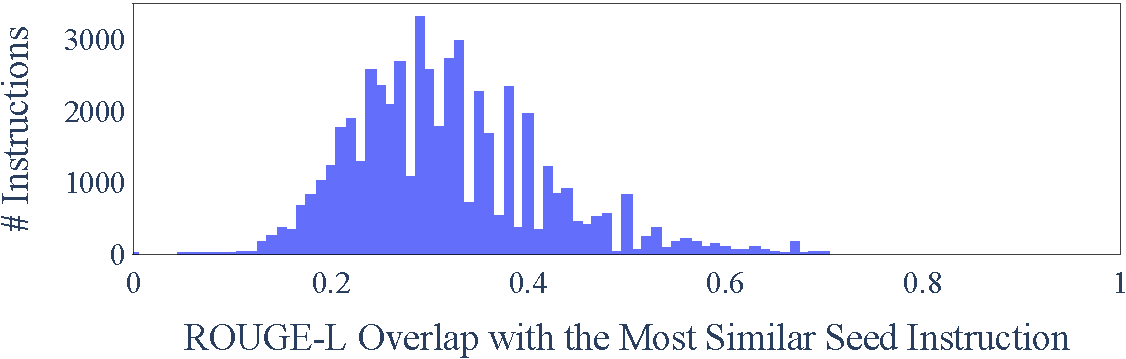
\includegraphics[width=\linewidth]{figures/overlap_with_seed_instructions.pdf}
    \end{subfigure}
    \caption{Distribution of the ROUGE-L scores between generated instructions and their most similar seed instructions. \label{fig:overlap-distribution}}
    \par\bigskip
    \begin{subfigure}{0.99\linewidth}
      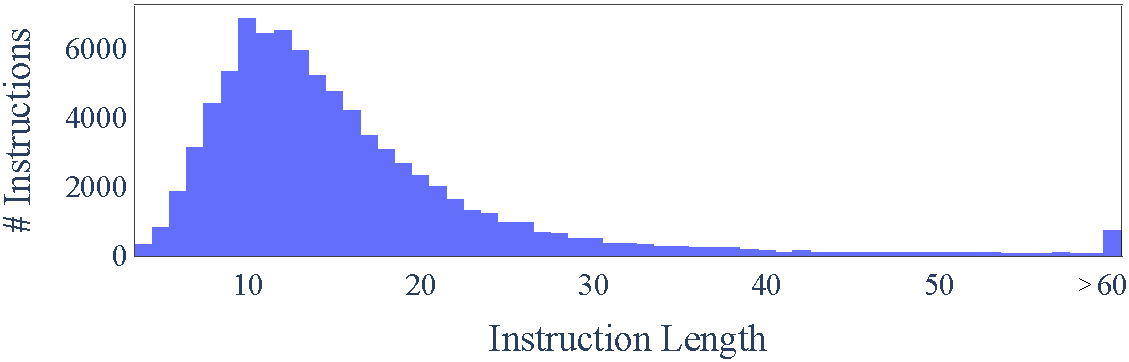
\includegraphics[width=\linewidth]{figures/instruction_length.pdf}
    \end{subfigure}
    \par\medskip
    \begin{subfigure}{0.99\linewidth}
      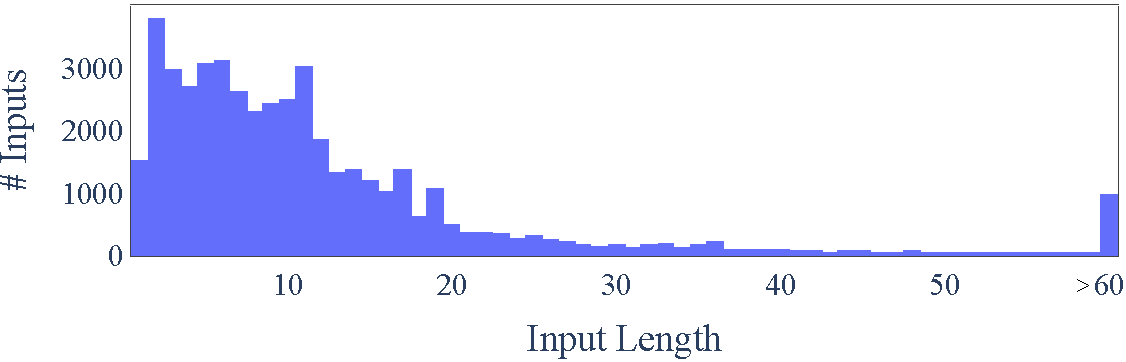
\includegraphics[width=\linewidth]{figures/input_length.pdf}
    \end{subfigure}
    \par\medskip
    \begin{subfigure}{0.99\linewidth}
      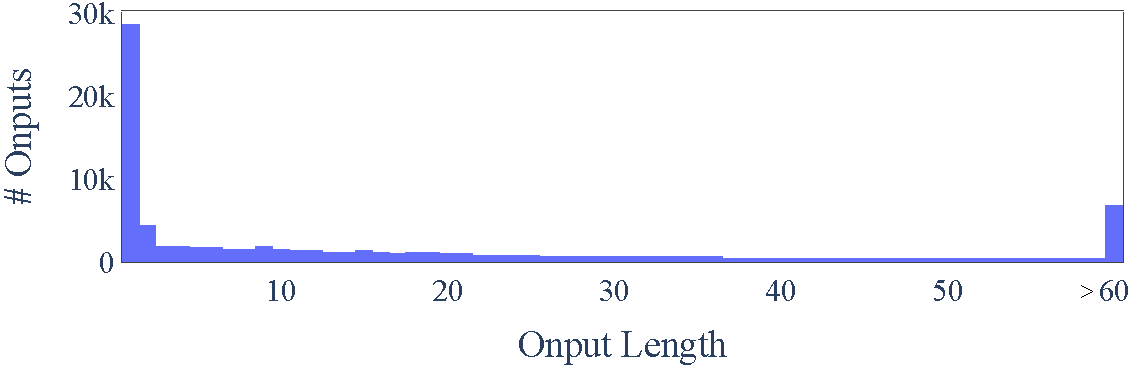
\includegraphics[width=\linewidth]{figures/output_length.pdf}
    \end{subfigure}
    \caption{Length distribution of the generated instructions, non-empty inputs, and outputs.  \label{fig:length_distribution}
  }
  \end{minipage}
  }

\end{figure*}

\section{\name{} Data from \gptthree{}}
\label{sec:generatd-data}

% So far, we have introduced our method of inducing instruction data from a pretrained language model. 
In this section, we apply our method for inducing instruction data to \gptthree{} as a case study. We use the largest GPT3 language model (``davinci'' engine) accessed through the OpenAI API\footnote{\url{https://openai.com/api/}}. The parameters for making queries are described in Appendix \ref{subsec:query_gpt3_api}. Here we present an overview of the generated data.

\subsection{Statistics}
\label{subsec:statistics}

\autoref{tab:data_statistics} describes the basic statistics of the generated data. We generate a total of over 52K instructions, and more than 82K instances corresponding to these instructions after filtering.
% \begin{figure*}[ht]
%   \adjustbox{valign=t}{
%   \begin{minipage}{0.55\linewidth}
%   \begin{subfigure}{\linewidth}
%     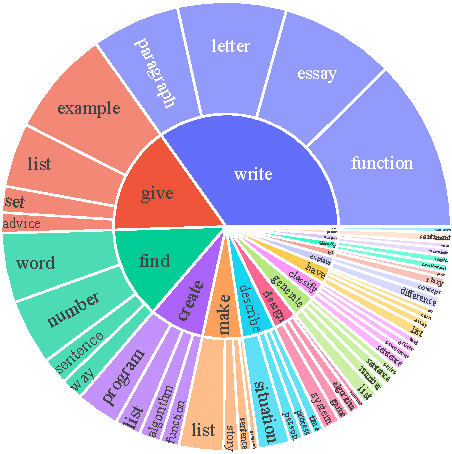
\includegraphics[width=\linewidth]{figures/instruction_sunburst_v2.pdf}
%     \caption{The top-20 most common root verbs (inner circle) and their top-4 direct noun objects (outer circle) in the generated instructions. Despite their diversity, the instructions shown here only account for 14\% of all the generated instructions because many instructions (e.g., ``Classify whether the user is satisfied with the service.'') do not contain such a verb-noun structure.}
%     \label{subfig:key-a}
%   \end{subfigure}\hfill
%   \end{minipage}
%   }
%   \hfill
%   \adjustbox{valign=t}{
%   \begin{minipage}{0.41\linewidth}
%     \vspace{10pt}
%     % \begin{subfigure}{0.475\linewidth}
%     %   \includegraphics[width=\linewidth]{figures/instruction_sunburst.pdf}
%     %   \caption{}\label{subfig:key-b}
%     % \end{subfigure}\hfill
%     \begin{subfigure}{0.95\linewidth}
%       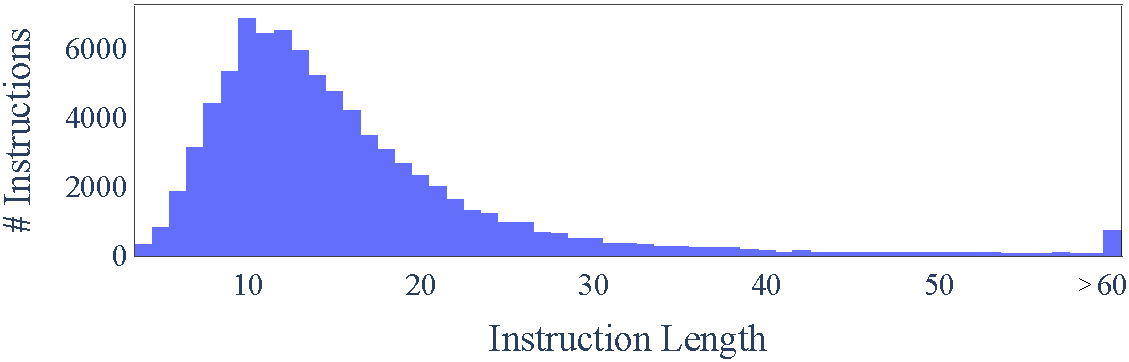
\includegraphics[width=\linewidth]{figures/instruction_length.pdf}
%       \caption{Distribution of instruction length (words)}\label{subfig:key-c}
%     \end{subfigure}
%     \medskip
%     \begin{subfigure}{0.95\linewidth}
%       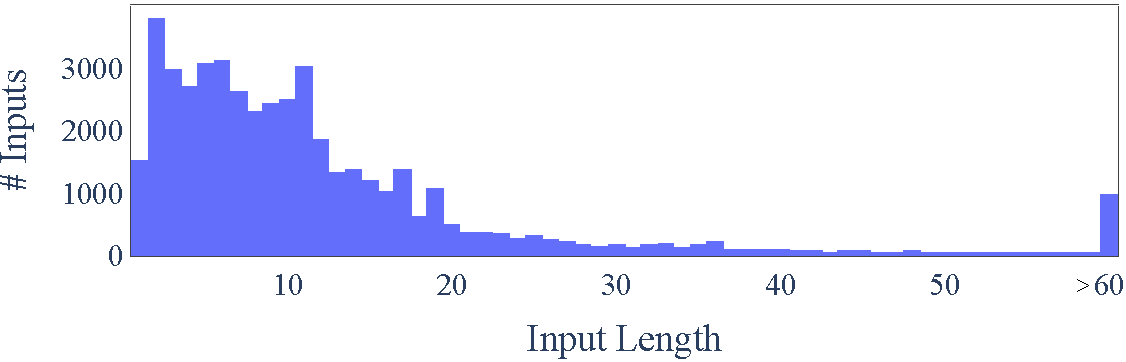
\includegraphics[width=\linewidth]{figures/input_length.pdf}
%       \caption{Distribution of non-empty input length (words)}\label{subfig:key-d}
%     \end{subfigure}\hfill
%     \begin{subfigure}{0.95\linewidth}
%       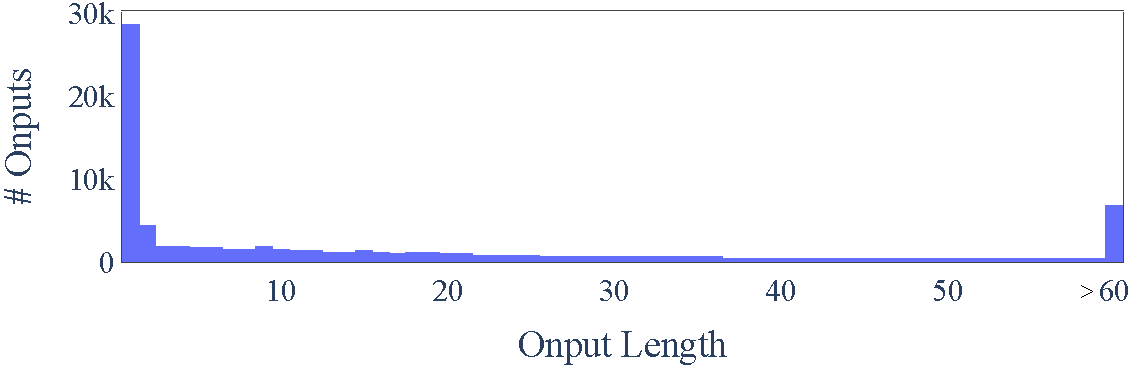
\includegraphics[width=\linewidth]{figures/output_length.pdf}
%       \caption{Distribution of output length (words)}\label{subfig:key-e}
%     \end{subfigure}\hfill
%   \end{minipage}
%   }
%   \caption{Distribution statistics of the generated instruction data. \todo{Make the font bigger. Make them different figures. Include a figure for the distance between generated instructions and their most similar seed tasks.}
%   % \daniel{state the unit of measurement (``token''?)} 
%   }
%   \label{fig:generated_data_distribution}
% \end{figure*}



\begin{figure*}[ht]
  \adjustbox{valign=t}{
  \begin{minipage}{0.55\linewidth}
    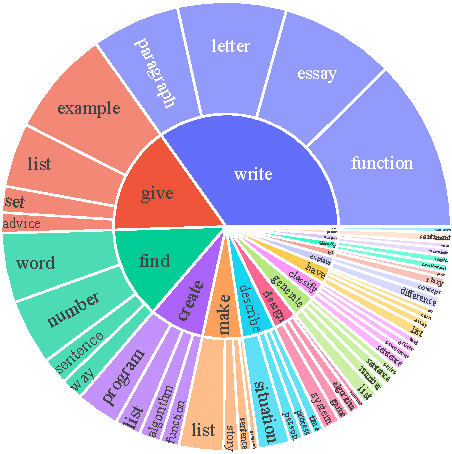
\includegraphics[width=0.98\linewidth,trim=0.5cm 0cm 0.35cm 0cm]{figures/instruction_sunburst_v2.pdf}
    \caption{The top 20 most common root verbs (inner circle) and their top 4 direct noun objects (outer circle) in the generated instructions. Despite their diversity, the instructions shown here only account for 14\% of all the generated instructions because many instructions (e.g., ``Classify whether the user is satisfied with the service.'') do not contain such a verb-noun structure. \label{fig:verb-noun-distribution}}
    \hfill
  \end{minipage}
  }
  \hfill
  \adjustbox{valign=t}{
  \begin{minipage}{0.4\linewidth}
   \begin{subfigure}{0.99\linewidth}
      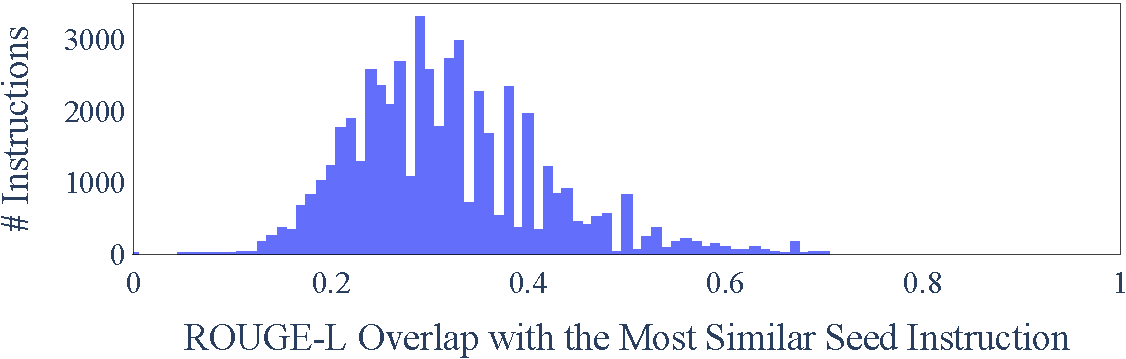
\includegraphics[width=\linewidth]{figures/overlap_with_seed_instructions.pdf}
    \end{subfigure}
    \caption{Distribution of the ROUGE-L scores between generated instructions and their most similar seed instructions. \label{fig:overlap-distribution}}
    \par\bigskip
    \begin{subfigure}{0.99\linewidth}
      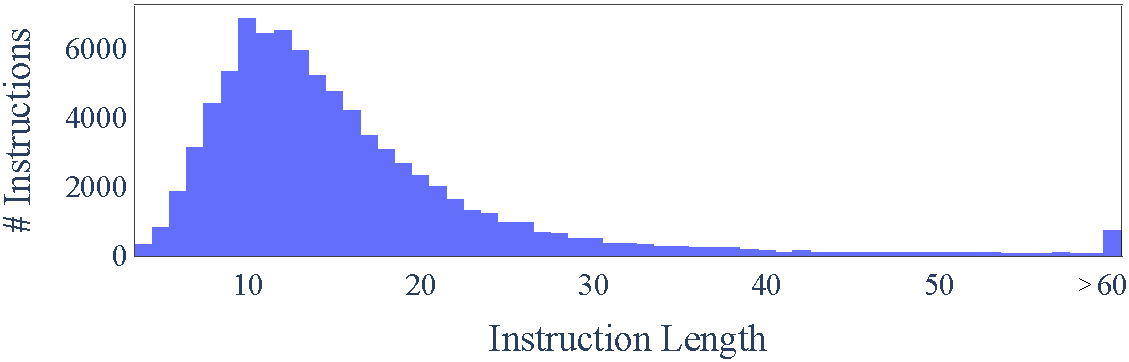
\includegraphics[width=\linewidth]{figures/instruction_length.pdf}
    \end{subfigure}
    \par\medskip
    \begin{subfigure}{0.99\linewidth}
      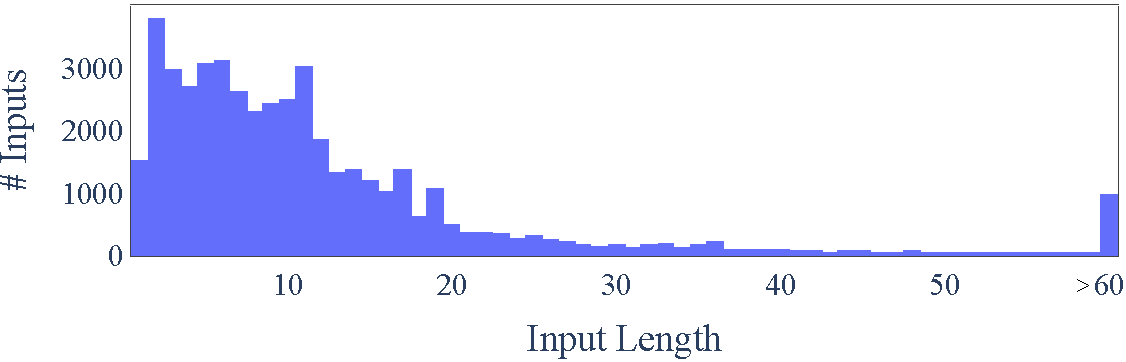
\includegraphics[width=\linewidth]{figures/input_length.pdf}
    \end{subfigure}
    \par\medskip
    \begin{subfigure}{0.99\linewidth}
      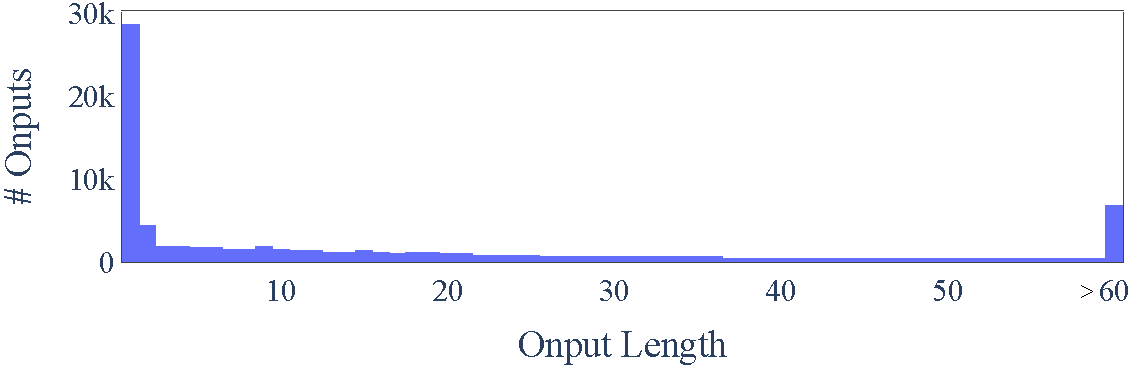
\includegraphics[width=\linewidth]{figures/output_length.pdf}
    \end{subfigure}
    \caption{Length distribution of the generated instructions, non-empty inputs, and outputs.  \label{fig:length_distribution}
  }
  \end{minipage}
  }

\end{figure*}

\subsection{Diversity}
\label{subsec:diversity}
To study what types of instructions are generated and how diverse they are, we identify the verb-noun structure in the generated instructions. We use the Berkeley Neural Parser\footnote{\url{https://parser.kitaev.io/}} \citep{kitaev-klein-2018-constituency,kitaev-etal-2019-multilingual} to parse the instructions, and then extract the verb that is closest to the root of the parse tree as well as its first direct noun object. 26,559 out of the 52,445 instructions contain such structure; other instructions usually contain more complex clauses (e.g., ``Classify whether this tweet contains political content or not.'') or are framed as questions (e.g., ``Which of these statements are true?''). 
We plot the top 20 most common root verbs and their top 4
direct noun objects in \autoref{fig:verb-noun-distribution}, which accounts for 14\% of the entire set. Overall, we see quite diverse intents and textual formats in these instructions.

We further study how the generated instructions differ from the seed instructions that are used to prompt the generation. For each generated instruction, we compute its highest ROUGE-L overlap with the 175 seed instructions. We plot the distribution of these ROUGE-L scores in \autoref{fig:overlap-distribution}, indicating a decent number of new instructions that do not have much overlap with the seeds. 
% \alisa{how to quantify what is ``much overlap''?}
We also demonstrate diversity in length of the instructions, instance inputs, and instance outputs in \autoref{fig:length_distribution}. 
% \alisa{what counts as ``diverse'' length?}

\subsection{Quality}
So far, we have shown the quantity and diversity of the generated data, but its quality remains uncertain. To investigate this, we randomly sample 200 instructions and randomly select 1 instance per instruction. We asked an expert annotator (co-author of this work) to label whether each instance is correct or not, in terms of the instruction, the instance input, and the instance output. 
% Table \ref{tab:data_quality_eval} lists the questions we ask the expert annotator, and to what proportion the evaluated field is valid. 
Evaluation results in \autoref{tab:data_quality_eval} show that most of the generated instructions are meaningful, while the generated instances may contain more noise (to a reasonable extent). However, we found that even though the generations may contain errors, most of them are still in the correct format or even partially correct, which can provide useful guidance for training models to follow instructions. We listed a number of good generations and bad generations in \autoref{tab:generated_tasks} and \autoref{tab:bad-generated-tasks} respectively.

\begin{table}[h]
\small
  \setlength\doublerulesep{\arrayrulewidth} % Daniel: to reduce the massive space between to back-to-back midrule's 
\centering
\begin{tabular}{|c|c|}
\toprule
Quality Review Question                                   & Yes \% \\ 
\midrule \midrule
\makecell[c]{Does the instruction \\ describe a valid task? }               &   92\%  \\ \midrule
\makecell[c]{Is the input appropriate \\ for the instruction?}               &   79\% \\ \midrule
\makecell[c]{Is the output a correct and acceptable \\ response to the instruction and input?} &   58\%  \\ \midrule
\midrule
All fields are valid                                        &  54\%   \\ \bottomrule
\end{tabular}
\caption{Data quality review for the instruction, input, and output of the generated data. See \autoref{tab:generated_tasks} and \autoref{tab:bad-generated-tasks} for representative valid and invalid examples.
% Review metadata is available here:  
% \href{https://docs.google.com/spreadsheets/d/1xkl-ohwzEZPvPK-Qy0alfmEcWNDe6jpulRzARWN9OqI/edit#gid=2123954903}{here}.
}
\label{tab:data_quality_eval}
\end{table}



\label{subsec:quality}



\section{Experimental Results}
% \section{Zero-shot Evaluation on NLP Tasks}
\label{sec:superni_results}

% \section{Experiments}
% \label{sec:exp}
% \paragraph{LM Eval Harness}
% \paragraph{PromptSource Tasks}
% \paragraph{T0 Eval}
% \paragraph{BigBench}
% \paragraph{EditEval}
% \paragraph{SuperNaturalInstructions}

We conduct experiments to measure and compare the quality of models under various instruction tuning setups. 
We first describe our models and other baselines, followed by our experiments. 

\subsection{\gptself{}: fine-tuning \gptthree{} on its own instruction data}
\label{subsec:self-instruct-gpt3}
% \daniel{
% Here or earlier: 
% We build \gpttself{} based on the data generated in S4.
% Need to flesh out hyper-parameters etc for this training.
% }
With the instruction-generated instruction data, we conduct instruction tuning for the \gptthree{} model itself (the ``davinci'' engine). As we described in \S\ref{subsec:instruction-tuning}, we use various templates to concatenate the instruction and input, and train the model to generate the output. This finetuning is done through the OpenAI finetuning API\footnote{\url{https://beta.openai.com/docs/guides/fine-tuning}}. We use the default hyper-parameters, except that we set the prompt loss weight to 0, and we train the model for 2 epochs. We refer the readers to Appendix~\ref{subsec:finetuning_details} for additional finetuning details. The resulting model is denoted as \gptself{}.

\subsection{Baselines}
% We compare our self-instructed GPT3 with several classes of baselines. 
\paragraph{Off-the-shelf language models.} 
We evaluate T5-LM \cite{lester2021power,raffel2020exploring} and \gptthree{}~\cite{brown2020gpt3} as the vanilla LM baselines (only pre-training, no additional fine-tuning). 
These baselines will indicate the extent to which off-the-shelf LMs are capable of following instructions naturally immediately after pretraining.

\paragraph{Publicly-available instruction-tuned models.}
\tzero{} and \tkinstruct{} are two instruction-tuned models proposed in \citet{sanh2022multitask} and \citet{wang2022benchmarking} respectively, and are demonstrated to be able to follow instructions for many NLP tasks. 
Both of these models are finetuned from the T5~\cite{raffel2020exploring} checkpoints and are publicly available\footnote{\url{https://huggingface.co/bigscience/T0}}\footnote{\url{https://huggingface.co/allenai/tk-instruct-11b-def}}. For both of these models, we use their largest version with 11B parameters.

\paragraph{Instruction-tuned GPT3 models.}
 We evaluate \gptinstruct{}~\cite{ouyang2022training}, 
which is developed by OpenAI based on GPT3 to follow human instructions better and has been found by the community to have impressive zero-shot abilities. 
There are various generations of these models,
where newer ones use more expansive data or algorithmic novelties\footnote{\url{https://beta.openai.com/docs/model-index-for-researchers}}.  
%based on various fine-tuning data or algorithms. 
For our \supernatShort{} experiments in \S\ref{subsec:superni-experiments}, we only compare with their \texttt{text-davinci-001} engine, because their newer engines are trained with the latest user data and are likely to already see the \supernatShort{} evaluation set. For our human evaluation of these models on newly written instructions, we include their 001, 002 and 003 engines for completeness.

Additionally, to compare \name{} training with other publicly available instruction tuning data, we further finetune GPT3 model with data from \promptsource{} and \supernatShort{}, which are used to train the \tzero{} and \tkinstruct{} models. We call them \tzero{} training and \supernatShort{} training for short, respectively. 
To save the training budget, we sampled 50K instances (but covering all their instructions) for each dataset, which has a comparable size to the instruction data we generated. Based on the findings from \citet{wang2022benchmarking} and our early experiments, reducing the number of instances per task does not degrade the model's generalization performance to unseen tasks.
% \alisa{this sounds suspicious... what is the size difference? were the original datasets much bigger?}
% Most of our experiments are based on their \texttt{text-davinci-001} engine, which is closest to our setup (see Footnote~\ref{footnote:gpt:instruct}). 



\subsection{Experiment 1: Zero-Shot Generalization on \supernatShort{} benchmark}
\label{subsec:superni-experiments}
We first evaluate the models' ability to follow instructions on typical NLP tasks in a zero-shot fashion. 
% We use \supernat{}~\cite{wang2022benchmarking} (\supernatShort{} in short) for evaluating models' ability to solve typical NLP tasks by following instructions. 
We use the evaluation set of \supernatShort{} ~\cite{wang2022benchmarking}, which consists of 119 tasks with 100 instances in each task. 
% There are a total of 11,810 instances in this evaluation set.
In this work, we mainly focus on the zero-shot setup, i.e., the model is prompted with the definition of the tasks only, without in-context demonstration examples.
For all our requests to the \gptthree{} variants, we use the deterministic generation mode (temperature as 0 and no nucleus sampling) without specific stop sequences.

% The evaluation set of \supernatShort{} contains 119 tasks in 12 categories, with 100 instances in each task.

\newcommand{\xbias}{-70ex}

\begin{table*}[ht]
\centering
\small
{\renewcommand{\arraystretch}{1.15}%
\begin{tabular}{lcc}
\toprule
\textbf{Model}                                                   & \textbf{\# Params}            & \textbf{ROUGE-L} \\
\midrule
\textbf{Vanilla LMs}                                                    \\
T5-LM                                                            & 11B                           & 25.7                                            \\
\tikzmark{a} {\color{black} \gptthree{}}                                                            & 175B                          & 6.8                                                 \\
\midrule

\textbf{Instruction-tuned w/o {\color{black}\supernatShort}}                    \\
\tzero                                                               & 11B                           & 33.1                                                \\
{\color{black} \gptthree{}} + \tzero{} Training                                               & 175B                          & 37.9                                                \\
\tikzmark{b}\tikzmark{c}{\color{black} \gptself{} }
% := \gptthree{}} + {\color{purple}\name{}} 
(Ours)                            & 175B                          & 39.9                                                \\
\tikzmark{d}{\color{black}\gptinstruct{001}}                                   & 175B                          & \textbf{40.8}                                                \\
\midrule

\textbf{Instruction-tuned w/ {\color{black}\supernatShort}}             \\
\tkinstruct{}                                                      & 11B                           & 46.0                                                  \\
\tikzmark{f}{\color{black} \gptthree{}} + {\color{black}\supernatShort{}} Training                                          & 175B                          & 49.5                                                \\
\tikzmark{e}{\color{black} \gptself{}}
% {\color{DarkBlue} \gptthree{}} + {\color{purple}\name{}} + 
+ {\color{black}\supernatShort{}} Training   (Ours)       & 175B                          & \textbf{51.6} \\
\bottomrule
\end{tabular}
\begin{tikzpicture}[ remember picture, overlay]
    \draw [<->]  ([yshift=1.1ex,xshift=-0.5ex]pic cs:b) [bend left=40] to ([yshift=0.1ex,xshift=-0.5ex, looseness=2]pic cs:a);
    \node at (\xbias,2.8ex) {\textcircled{\tiny 1}};
    \draw [<->]  ([yshift=0.3ex,xshift=-0.5ex]pic cs:d) [bend left=90] to ([yshift=0.6ex,xshift=-0.5ex, looseness=2]pic cs:c);
    \node at (\xbias,-4.0ex) {\textcircled{\tiny 2}};
    % \draw [<->]  ([yshift=0.3ex,xshift=-0.5ex]pic cs:e) [bend left=90] to ([yshift=0.6ex,xshift=-0.5ex, looseness=2]pic cs:f);
    \draw [<->]  ([yshift=0.3ex,xshift=-0.5ex]pic cs:e) [bend left=90] to ([yshift=0.6ex,xshift=-0.5ex, looseness=2]pic cs:f);
    \node at (\xbias,-17.7ex) {\textcircled{\tiny 3}};
\end{tikzpicture}
\caption{Evaluation results on \emph{unseen} tasks from {\color{black}\supernat{}} (\S\ref{subsec:superni-experiments}). 
From the results, we see that \textcircled{\tiny 1}  \name{} can boost \gptthree{} performance by a large margin (+33.1\%) and \textcircled{\tiny 2} nearly matches the performance of \gptinstruct{001}. 
Additionally, \textcircled{\tiny 3} it can further improve the performance even when a large amount of labeled instruction data is present. 
% \hanna{what is instrctGPT-openAI on instruction-tuned with sup-natinst}\yizhong{that's the old naming. I updated them.}
}
\label{tab:superni_results}
}
\end{table*}
\begin{figure*}[t!]
    \centering
    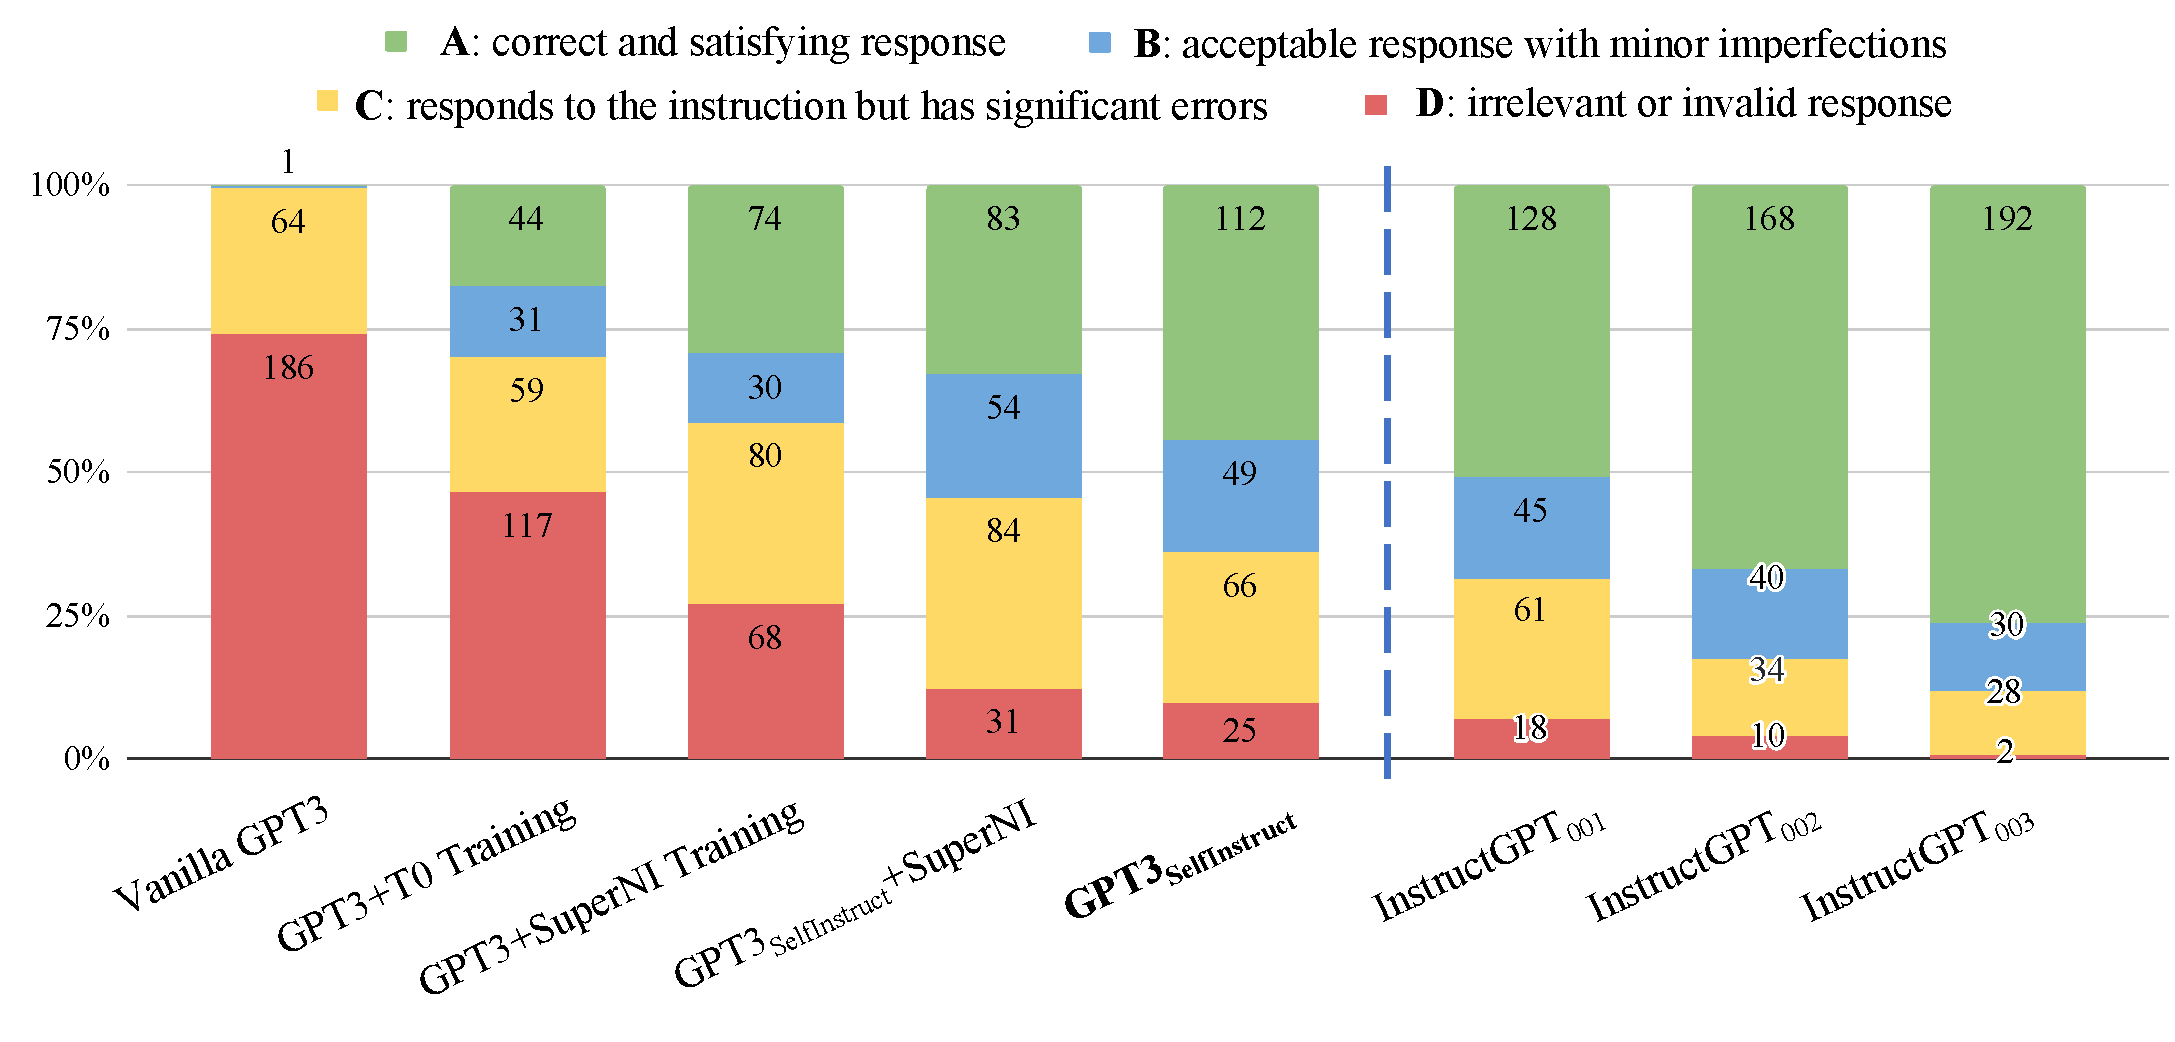
\includegraphics[width=\textwidth, trim={0 20 0 10}]{figures/human_instruction_results.pdf}
    \caption{
    Performance of GPT3 model and its instruction-tuned variants, evaluated by human experts on our 252 user-oriented instructions (\S\ref{sec:user_instructions}). Human evaluators are instructed to rate the models' responses into four levels.
    % \daniel{Added this; check if it is right:}
    The results indicate that \gptself{} outperforms 
    all the other \gptthree{} variants trained on publicly available instruction datasets. 
    Additionally, \gptself{} scores nearly as good as \gptinstruct{001} (c.f., \autoref{footnote:gpt:instruct}).
    }
    \label{fig:human_instructions_results}
\end{figure*}

\paragraph{Results.}
% Table~\ref{tab:superni_results} compares the performance of different models on the evaluation set of \supernatShort{}. 
We make the following observations from the results in \autoref{tab:superni_results}. 
\name{} 
% significantly \nascomment{do not use the word `significantly' if you did not do a significance test!}  
boosts the instruction-following ability of \gptthree{} by a large margin. The vanilla \gptthree{} model basically cannot follow human instructions at all. Upon manual analysis, we find that it usually generates irrelevant and repetitive text, and does not know when to stop generation. 
Compared with other models that are not specifically trained for \supernatShort{}, \gptself{} achieves better performance than \tzero{} or the \gptthree{} finetuned on the \tzero{} training set, which takes tremendous human labeling efforts. Notably, \gptself{} also nearly matches the performance of \gptinstruct{001}, which is trained with private user data and human-annotated labels.

Models trained on \supernatShort{} training set still achieve better performance on its evaluation set, which we attribute to the similar instruction style and formatting. However, we show that \name{} still brings in additional gains when combined with the \supernatShort{} training set, proving its value as complementary data. 
% We will show that models trained with \name{} demonstrate even more broad \nascomment{what does `broad' mean here?  cut it} instruction following than those trained on with T0 or \supernatShort{} in Section \ref{sec:user_instructions}.



\subsection{Experiment 2: Generalization to User-oriented Instructions on Novel Tasks}
\label{sec:user_instructions}

Despite the comprehensiveness of \supernatShort{} in collecting existing NLP tasks, most of these NLP tasks were proposed for research purposes and skewed toward classification. To better access the practical value of instruction-following models, a subset of the authors curate a new set of instructions motivated by user-oriented applications. 
% These instructions are newly written by three of our co-authors. 
We first brainstorm different domains where large LMs may be useful (e.g., email writing, social media, productivity tools, entertainment, programming), then craft instructions related to each domain along with an input-output instance (again, input is optional). We aim to diversify the styles and formats of these tasks (e.g., instructions may be long or short; input/output may take the form of bullet points, tables, codes, equations, etc.). In total, we create 252 instructions with 1 instance per instruction. We believe it can serve as a testbed for evaluating how instruction-based models handle diverse and unfamiliar instructions. \autoref{tab:case_study} presents a small portion of the 252 tasks. The whole test set will be available upon request.

% The current benchmarks for evaluating models often do not accurately reflect user  needs or instructions found in real-world applications. In order to better assess the practical value of NLP models, we propose a new benchmark for evaluating their ability to generalize to user-oriented instructions. This benchmark consists of a collection of instructions from real-world applications such as productivity, writing, and collaboration tools, as well as social media and entertainment applications. These instructions cover a wide range of tasks, styles, and formats commonly found in real-world settings and provide a more challenging testbed for NLP models. These instructions represent a diverse set of real-world tasks that NLP models may not have encountered during training, making them a valuable resource for evaluating the ability of NLP models to generalize to new and unfamiliar instructions. By assessing the performance of NLP models on these instructions, we can better understand their ability to handle the diverse and often open-ended tasks found in real-world applications. \nascomment{way too vague here.  I have no idea how you produced these instructions!  I remember talking about crowdsourcing this, but if you did that you need to give a lot more detail about what you asked people to do and why!}

\paragraph{Human evaluation setup.}
Evaluating models' performance on this evaluation set of diverse tasks is extremely challenging because different tasks require different expertise. Indeed, many of these tasks cannot be measured by automatic metrics or even be judged by normal crowdworkers (e.g., writing a program, or converting first-order logic into natural language). To get a more faithful evaluation, we asked the authors of the instructions to judge model predictions. The evaluators were asked to rate the output based on whether it accurately and effectively completes the task. We implemented a four-level rating system for categorizing the quality of the models' outputs, defined as follows:

\begin{itemize}[noitemsep, leftmargin=*]
    \item \textsc{Rating-A:} The response is valid and satisfying.
    \item \textsc{Rating-B:} The response is acceptable but has minor errors or imperfections that can be improved.
    \item \textsc{Rating-C:} The response is relevant and responds to the instruction, but it has significant errors in the content. For example, GPT3 might generate a valid output first, but continue to generate other irrelevant things.
    \item \textsc{Rating-D:} The response is irrelevant or invalid, including repetition of the input, totally irrelevant output, etc.
\end{itemize}

% Level 1 indicates that the response is irrelevant or invalid, such as a repetition of the input or totally irrelevant output. Level 2 indicates that the response is relevant and responds to the instruction, but contains significant errors in the content, for example, the model generates a valid output first but continues to generate other irrelevant responses. Level 3 indicates that the response is acceptable but has minor errors or imperfections that could be improved. Finally, Level 4 indicates that the response is valid and satisfying. This four-level system allowed us to systematically evaluate the performance of models on the user-oriented instructions and provided a detailed understanding of the model's capabilities and limitations.



%\todo{One paragraph describing how we set up the human evaluation, and what we evaluate. If we have an interface, let's include it in the appendix.}
%To encourage the practical value of these instruction-based models, we can come up instructions from the perspective of real-world applications (e.g., Grammarly, MS Office, Google docs, \url{https://ludwig.guru/}, Yelp, LinkedIn, Amazon, Netflix, Overleaf, Spotify). E.g., for Spotify, we can write instructions such as "Recommend 10 songs to listen during road trip."
%Ask Yeganeh to come up with 50 applications, and think of tasks in these applications, write instructions \& instances.
%Aiming for 500 instructions and instances written by experts. 
%Human evaluation to get the performance.
\paragraph{Results.}
\autoref{fig:human_instructions_results} provides the performance of \gptthree{} model and its instruction-tuned counterparts on this newly written instruction set. As anticipated, the vanilla \gptthree{} language model is largely unable to respond to instructions, and all instruction-tuned models demonstrate comparatively higher performance, 
% In most cases, the model simply repeats the input and cannot stop its generation until it reaches the generation length limit. 
% Consistent with the previous experiment on \supernatShort{} the \name{} significantly enhanced the performance of the GPT3 model.
% All instruction-tuned models demonstrate a better ability than \gptthree{} to follow these newly written testing instructions. 
Nonetheless, \gptself{} (i.e.,  \gptthree{} model fine-tuned with \name) outperforms those counterparts trained on \tzero{} or \supernatShort{} by a large margin, demonstrating the value of the generated data despite the noise. 
Compared with \gptinstruct{001} (c.f. \autoref{footnote:gpt:instruct}), \gptself{} is quite close in the performance---if we count acceptable response with minor imperfections (\textsc{Rating-3}) as valid, \gptself{} is only 5\% behind \gptinstruct{001}. Lastly, our evaluation confirms the impressive instruction-following ability of \gptinstruct{002} \& \gptinstruct{003} models. Although there are many factors behind this success, we conjecture that future work can largely benefit from improving the quality of our generated data by using human annotators or training a reward model to select better generations, similar to the algorithm used in \citet{ouyang2022training}.
% \alisa{need to emphasize how much less resources was required for self-instruct.}

% Also, it outperformed the models trained on the labeled data (T0 Training and \supernatShort{} Training). Our results demonstrate that \gptself{} achieves a performance that is comparable to that of the \gptinstruct{001} model, although there is still a large gap from the \gptinstruct{002} and \gptinstruct{003} models.
% \name{} performed better than the model trained on \name{} and \supernatShort{}. We conjecture that the observed results may be attributed to the preponderance of classification tasks in \supernatShort{}. 

%\nascomment{from here you start calling it ``self-instructing'' but I thought the name was self-instruct (with smallcaps) ... be consistent!} 

\subsection{Example Predictions from \gptself{}}
\label{sec:example-predictions}
% \subsection{Case study} \nascomment{I think you should retitle this section ``Examples''}
% To provide a more intuitive sense of how good our model is in following instructions and what is its limitation, 
We present a selection of user-oriented tasks, the corresponding \gptself{}-produced responses and annotator ratings in \autoref{tab:case_study}. %The tasks include queries about making a decision, work management, and logical inference. 
% Overall, these are many cases we found the \gptself{} model provides acceptable or even satisfying responses. 
We see that even for responses rated as level 2, the model demonstrates extensive steps in solving the task, even though its final output is incorrect. 
% While the \name{} model was able to accurately provide the requested information for most tasks, there were some instances in which errors were observed. 
% Despite these errors, the overall performance of the \name{} model demonstrates it is effective in handling user-oriented tasks.
\setlength\tabcolsep{1 pt} % to reduce the margin of the table
\newcommand{\sep}{-0.1cm} % separation between elements of itemize
\newcommand{\sty}{\tt \scriptsize}
\renewcommand\labelitemi{--} % change the label of itemize to "-" 

\newcommand{\ins}{{\greentext{Instruction:}}}
\newcommand{\inp}{\newline{\greentext{Input:}}}

\begin{table*}[th!]
\centering
\small
\resizebox{1\textwidth}{!}{
\begin{tabular}{p{0.29\textwidth}|p{0.40\textwidth}|p{0.32\textwidth}|c}
\toprule
\multicolumn{1}{c}{\textbf{Instruction + Instance Input}}   & \multicolumn{1}{c}{\textbf{Target Response}} & \multicolumn{1}{c}{\textbf{\gptself{} Response}}   & \multicolumn{1}{c}{\textbf{Rating}}\\
\midrule
\sty
\ins{} Give students tips on how to keep their nerves under control during class presentations. &  
\sty
Everyone gets a little nervous when speaking in front of a group. That’s normal. But the more preparation you’ve done—meaning plenty of researching, organizing, and rehearsing—the more confident you’ll be. Preparation is the key. And if you make a mistake or stumble over your words, just regroup and keep going. Nobody’s perfect, and nobody expects you to be. & 
\vspace{-2mm}
\sty
\begin{itemize}[leftmargin=0.3cm, itemsep=\sep, topsep=0.1pt]
    \item Practice your presentation in front of friends and family. 
    \item Don't drink too much caffeine before the presentation. 
    \item Take deep breaths before you start speaking. 
    \item If you feel nervous, smile. 
    \item Remember that everyone in the audience is rooting for you. 
\end{itemize} & \sty A
\\
\midrule
\sty
\ins{} Make a list of the pros and cons of the given decision. 
\inp{} Implementing a Remote Working Policy 
& 
\sty
Pros: \begin{itemize}[leftmargin=0.3cm, itemsep=\sep, topsep=0.1pt]
    \item Allowing employees to work from home can reduce their stressful commutes and increase their productivity.
    \item Remote working provides greater flexibility, particularly for working parents and caregivers who have other responsibilities. 
    % \item It's possible to hire highly creative people who live further away if they don't have to come into the office every day.
    % \item People who aren't distracted by office noises and regular interruptions will perform better. 
    % \item Team members' communication skills will improve, as they will learn to communicate more effectively using email and IM, for example. 
    \item \dots (more points)
\end{itemize}

Cons:
\begin{itemize}[leftmargin=0.3cm, itemsep=\sep, topsep=0.1pt]
    \item It may be more difficult for team members to build meaningful, productive, creative relationships with one another.    
    \item \dots (more points)
    \end{itemize}
    &  
    \sty
    Pros:
\begin{itemize}[leftmargin=0.3cm, itemsep=\sep, topsep=0.1pt]
    \item Employees can work from home and save on commuting costs.     
    \item Employees can spend more time with their families.    
\end{itemize}
Cons:
\begin{itemize}[leftmargin=0.3cm, itemsep=\sep, topsep=0.1pt]   
    \item Employees may not be as productive as they would be in the office.    
    \item Employees may not be as motivated to work. 
\end{itemize} & \sty A
\\
\midrule
\sty
\ins{} A color description has been provided. Find the CSS code associated with that color. 
\inp{} A light red color with a medium light shade of pink & 
\sty
\#DB7093 ($\textcolor[HTML]{DB7093}\lgblksquare$)& 
\sty
~\#ff66cc ($\textcolor[HTML]{ff66cc}\lgblksquare$) & \sty B \\
%\yeganeh{Yizhong I don't think it's correct. the generated color is rose pink, while we are looking for a shade of pale red} \yizhong{yeah it seems we can rate this a level-3 if not 4?} \yeganeh{Yes}
\midrule

\sty
\ins{} Give some examples of what people usually say in the given social situation.  
\inp{} when someone arrives safely &
\sty
\vspace{-2mm}
\begin{itemize}[leftmargin=0.3cm, itemsep=\sep, topsep=0.1pt]
    \item ``Glad you made it safe and sound.''
    \item ``Good to see you got here unscathed.''
    \item ``So, bulletproof vests actually work!''
\end{itemize} 
&  
\sty
Thank God, I made it. & \sty B\\
\midrule
\sty
\ins{} You are given a sentence in first-order logic. Translate it into natural language.  
\inp{}
$\exists x \forall	y (soldier(x) $ 
$\to general(x,y))$ 
& 
\sty
There is someone (x) such that if he is a soldier, then he is general of everyone. &  
\sty
There exists a soldier such that for every general, he is a general. & \sty C\\
\midrule 
\sty 
\ins{}
Design an outline for a blog post based on the given information and list the sections accordingly. 
\inp{}
 This blog post is going to about making a list of last-minute gift ideas. Also, the tone of the post is going to be relaxed and casual. & 
\sty \begin{itemize}[leftmargin=0.3cm, itemsep=\sep, topsep=0 pt]
%\item Section: Gift card to a favorite restaurant or store
\item Section: Movie tickets
\item Section: A fun game console
%Section: Books 
%Section: Candles, flameless candles
%Section: Portable battery charger for phones/tablets
%Section: Water filter pitcher
\item Section: Personalized items with photos/artwork
\item ...(more sections)
%Section: Favorite team gear (hat, sweatshirt)
\item Takeaway: Don't stress about out running out of time to buy, make a gift. \end{itemize}&
\sty \begin{itemize}[leftmargin=0.3cm, itemsep=\sep, topsep=0 pt]
\item Introduction 
\item List of Gift Ideas
\item Conclusion \end{itemize}
& \sty C
 \\
\midrule
\sty
\ins{}
Write a Jira ticket for the given task. 
\inp{}
New Employee onboarding & 
\sty
Title: Please help our new employee get settled.
Prepare a desk, chair, and computer for them to use.
Create their company account, email, and temporary password.
Grant access to company documents. & 
\sty
Hi [Manager],
I’m writing to you because I have a question about the new employee onboarding process. I’ve been working here for a few months now, and I’m still not sure how it works. Could you please explain it to me? & \sty D\\
\midrule
\sty 
\ins{}
Create alliterations by finding synonyms for words in the given sentence. 
\inp{}
David wears a hat everyday. & \sty David dons a derby daily. & \sty  David wears a hat every day. & \sty D \\
\bottomrule
\end{tabular}
}
\caption{Examples in the User-oriented Instructions dataset (\S\ref{sec:user_instructions}) and predictions from \gptself{}. %\todo{Include more tasks (rating 1-4), sorted by rating.}
% \todo{explain what ratings are; add reference to the corresponding section.}
% \daniel{check this:}
The right column indicates one of the four quality ratings assigned to the model's response, with ``A'' indicating  ``valid and satisfying'' responses (highest)
and  ``D'' indicating ``irrelevant or invalid response'' (lowest).
}
\label{tab:case_study}
\end{table*}



\begin{comment}
\begin{table*}[th!]
\centering
\small
\resizebox{1\textwidth}{!}{
\begin{tabular}{p{0.15\textwidth}|p{0.13\textwidth}|p{0.33\textwidth}|p{0.3\textwidth}|c}
\toprule
\multicolumn{1}{c}{\textbf{Instruction}}  & \multicolumn{1}{c}{\textbf{Input}}  & \multicolumn{1}{c}{\textbf{Target}} & \multicolumn{1}{c}{\textbf{\gptself{} Response}}   & \multicolumn{1}{c}{\textbf{Rating}}\\
\midrule
\sty
Give students tips on how to keep their nerves under control during class presentations. & & 
\sty
Everyone gets a little nervous when speaking in front of a group. That’s normal. But the more preparation you’ve done—meaning plenty of researching, organizing, and rehearsing—the more confident you’ll be. Preparation is the key. And if you make a mistake or stumble over your words, just regroup and keep going. Nobody’s perfect, and nobody expects you to be. & 
\vspace{-2mm}
\sty
\begin{itemize}[leftmargin=0.3cm, itemsep=\sep, topsep=0.1pt]
    \item Practice your presentation in front of friends and family. 
    \item Don't drink too much caffeine before the presentation. 
    \item Take deep breaths before you start speaking. 
    \item If you feel nervous, smile. 
    \item Remember that everyone in the audience is rooting for you. 
\end{itemize} & \sty 4
\\
\midrule
\sty
Make a list of the pros and cons of the given decision. & 
\sty
Implementing a Remote Working Policy & 
\sty
Pros: \begin{itemize}[leftmargin=0.3cm, itemsep=\sep, topsep=0.1pt]
    \item Allowing employees to work from home can reduce their stressful commutes and increase their productivity.
    \item Remote working provides greater flexibility, particularly for working parents and caregivers who have other responsibilities. 
    % \item It's possible to hire highly creative people who live further away if they don't have to come into the office every day.
    % \item People who aren't distracted by office noises and regular interruptions will perform better. 
    % \item Team members' communication skills will improve, as they will learn to communicate more effectively using email and IM, for example. 
    \item \dots (more points)
\end{itemize}

Cons:
\begin{itemize}[leftmargin=0.3cm, itemsep=\sep, topsep=0.1pt]
    \item It may be more difficult for team members to build meaningful, productive, creative relationships with one another.    
    \item \dots (more points)
    \end{itemize}
    &  
    \sty
    Pros:
\begin{itemize}[leftmargin=0.3cm, itemsep=\sep, topsep=0.1pt]
    \item Employees can work from home and save on commuting costs.     
    \item Employees can spend more time with their families.    
\end{itemize}
Cons:
\begin{itemize}[leftmargin=0.3cm, itemsep=\sep, topsep=0.1pt]   
    \item Employees may not be as productive as they would be in the office.    
    \item Employees may not be as motivated to work. 
\end{itemize} & \sty 4
\\
\midrule
\sty
A color description has been provided. Find the CSS code associated with that color. & 
\sty
A light red color with a medium light shade of pink & 
\sty
\#DB7093 ($\textcolor[HTML]{DB7093}\lgblksquare$)& 
\sty
~\#ff66cc ($\textcolor[HTML]{ff66cc}\lgblksquare$) & \sty 3 \\
%\yeganeh{Yizhong I don't think it's correct. the generated color is rose pink, while we are looking for a shade of pale red} \yizhong{yeah it seems we can rate this a level-3 if not 4?} \yeganeh{Yes}
\midrule

\sty
Give some examples of what people usually say in the given social situation. & 
\sty
when someone arrives safely &
\sty
\vspace{-2mm}
\begin{itemize}[leftmargin=0.3cm, itemsep=\sep, topsep=0.1pt]
    \item ``Glad you made it safe and sound.''
    \item ``Good to see you got here unscathed.''
    \item ``So, bulletproof vests actually work!''
\end{itemize} 
&  
\sty
Thank God, I made it. & \sty 3\\
\midrule
\sty
You are given a sentence in first-order logic. Translate it into natural language. & 
\sty
$\exists x \forall	y (soldier(x) $ 
$\to general(x,y))$ 
& 
\sty
There is someone (x) such that if he is a soldier, then he is general of everyone. &  
\sty
There exists a soldier such that for every general, he is a general. & \sty 2\\
\midrule 
\sty Design an outline for a blog post based on the given information and list the sections accordingly. &
\sty This blog post is going to about making a list of last-minute gift ideas. Also, the tone of the post is going to be relaxed and casual. & 
\sty \begin{itemize}[leftmargin=0.3cm, itemsep=\sep, topsep=0 pt]
%\item Section: Gift card to a favorite restaurant or store
\item Section: Movie tickets
\item Section: A fun game console
%Section: Books 
%Section: Candles, flameless candles
%Section: Portable battery charger for phones/tablets
%Section: Water filter pitcher
\item Section: Personalized items with photos/artwork
\item ...(more sections)
%Section: Favorite team gear (hat, sweatshirt)
\item Takeaway: Don't stress about out running out of time to buy, make a gift. \end{itemize}&
\sty \begin{itemize}[leftmargin=0.3cm, itemsep=\sep, topsep=0 pt]
\item Introduction 
\item List of Gift Ideas
\item Conclusion \end{itemize}
& \sty 2
 \\
\midrule
\sty
Write a Jira ticket for the given task. & 
\sty
New Employee onboarding & 
\sty
Title: Please help our new employee get settled.
Prepare a desk, chair, and computer for them to use.
Create their company account, email, and temporary password.
Grant access to company documents. & 
\sty
Hi [Manager],
I’m writing to you because I have a question about the new employee onboarding process. I’ve been working here for a few months now, and I’m still not sure how it works. Could you please explain it to me? & \sty 1\\
\midrule
\sty Create alliterations by finding synonyms for words in the given sentence. & \sty David wears a hat everyday. & \sty David dons a derby daily. & \sty  David wears a hat every day. & \sty 1 \\
\bottomrule
\end{tabular}
}
\caption{Examples in the User-oriented Instructions dataset and predictions from \gptself{}. %\todo{Include more tasks (rating 1-4), sorted by rating.}
}
\label{tab:case_study}
\end{table*}
\end{comment}


%\todo{Yeganeh, could you create a big table with perfect generations from the self-instructing model, as well as some error examples where the model demonstrates some typical mistakes? All predictions are here:
% \href{https://docs.google.com/spreadsheets/d/1Cl69ki30Hfr90hMEzm2GqF4Fx2TAKZqJZL-Qfm_d758/edit#gid=702154844}{here}}


% \subsection{Effectiveness across Models}
% Try GPT-J (smaller size, openness) and T5-LM (encoder-decoder architecture).


% \section{Effect of Instruction Data Size}

% For data size, we need to plot the performance change against the number of generated instructions.

% For data quality, we can use the quality annotations from \ref{subsec:quality} and only use the high-quality instances for instruction tuning.

\section{Discussion and Limitation}

\subsection{Why does \name{} work?}
It is worthwhile to  reflect on the role that high-quality human feedback plays 
% the fundamentals that have  
in enabling the recent successes on instruction-tuning LMs~\cite{mishra2022cross,wang2022benchmarking,wei2022finetuned,sanh2022multitask,ouyang2022training}. 
% Fundamentally what do these models learn from observing human-annotated instructions? 
Here are two extreme hypotheses: 

\newcommand{\subscript}[2]{$#1 _ #2$}
\begin{enumerate}[label=(\subscript{H}{{\arabic*}})]
    \item  \emph{Human feedback} is a \emph{necessary and indispensable} aspect of instruction-tuning as LMs need to learn about issues that were not quite learned during pre-training. 
    % LMs learn about tasks and how to address them from human feedback. 
    % In other words, models learn about aspects of language that is not quite learned during pre-training and hence instruction-tuning with human-feedback is an indispensable step.   
    \item  \emph{Human feedback} is an \emph{optional} aspect of instruction-tuning as LMs are already quite familiar with instructions  from their pre-training. Observing the human feedback is merely a lightweight process for aligning their pre-training distribution/objective which might be replaceable with a different process. 
\end{enumerate}
While the reality probably lies somewhere in between these two extremes, we conjecture 
% \nascomment{I think you should use the verb `conjecture' -- hypothesize suggests that you're going to carry out an experiment to test it, which you don't do} 
that it is closer to \subscript{H}{2}, particularly for larger models.
This intuition, that LMs already know much about language instructions, is a key motivation for \name{} and is also supported by its  empirical success.


\subsection{Broader Impact}

Beyond the immediate focus of this paper, we believe that \name{} may help bring more transparency to what happens ``behind the scenes'' of widely-used instruction-tuned models like \gptinstruct{}. 
% \nascomment{rest of this paragraph is too wordy and repetitive.  rework to make the point concisely.} \alisa{took a stab at it}
% The parameters of these models and their training data remain hidden, limiting research progress that might otherwise prosper.
% Unfortunately, such industrial models remain behind the API walls as their datasets are not released, and hence there is little understanding of their constructions. There is no doubt that such a lack of transparency is not conducive to productive research progress.
% Now the burden falls on the shoulders of academia to better understand the source of success in these models and strive for even better, yet open, models.
Unfortunately, such industrial models remain behind the API walls as their datasets are not released, and hence there is little understanding of their constructions and why they demonstrate impressive capabilities.
% These industrial models remain behind the API walls and their datasets are not released. 
% There is no doubt that such lack of transparency is not conducive to productive research progress.
The burden now falls on academia to better understand the source of success in these models and strive for better -- yet open -- models. We believe our findings in this paper demonstrate the importance of diverse instruction data, and our large synthetic dataset can be the first step toward higher-quality data for building better instruction-following models.


% Better understanding various generations of GPT3Instruct 
% \todo{Discuss how instructGPT is trained - private user data and a lot of annotations blabla}
% \todo{Want to argue that we're isolating the algorithmic contribution from data contribution.} \yizhong{rewrote, check?}


\subsection{Limitations of \name}
Here, we discuss some limitations of this work to inspire future research in this direction.  

\paragraph{Tail phenomena.} 
\name{} depends on LMs, and it will inherit all the limitations that carry over with LMs. 
As recent studies have shown~\cite{razeghi2022impact,kandpal2022large},  \emph{tail phenomena} pose a serious challenge to the success of LMs. In other words, LMs' largest gains correspond to the frequent uses of languages (head of the language use distribution), and there are minimal gains in the low-frequency contexts. 
Similarly, in the context of this work, it would not be surprising if the majority of the gains by \name{} are skewed toward 
% popular \nascomment{I don't understand what makes a task  or instructions ``popular'' so I don't know what this means} 
tasks or instructions that present more frequently in the pre-training corpus. 
As a consequence, the approach might show brittleness with respect to uncommon and creative instructions.



\paragraph{Dependence on large models.} 
Because of \name's dependence on the inductive biases extracted from LMs, it might work best for larger models. 
If true, this may create barriers to access for those who may not have large computing resources. 
We hope future studies will carefully study the gains as a function of model size or various other parameters. 
It is worthwhile to note that instruction-tuning with human annotation also suffers from a similar limitation: gains of instruction-tuning are higher for larger model~\cite{wei2022finetuned}. 
% \daniel{Note: similar issue with human annotations }

\paragraph{Reinforcing LM biases.}
% It is very likely that A point of concern for the authors is whether \name{} 
% \nascomment{I don't understand what this sentence is trying to say.} The idea enabling \name{} is about iterative amplification of LM's inductive biases  \nascomment{ you seem to be mixing up ``inductive bias'' with stereotype kinds of biases.  don't do that} that pertain to instruction-following. 
A point of concern for the authors is the unintended consequences of this iterative algorithm, such as the amplification of problematic social biases (stereotypes or slurs about genders, races, etc.). 
Relatedly, one observed challenge in this process is the algorithm's difficulty in producing balanced labels, which reflected models' prior biases. 
We hope future work will hash out such details to better understand the pros and cons of the approach. 


 % \paragraph{Acceptability to LM poisoning.}

% \begin{itemize}
    % \item Some kills can never be learned
    % \item Some wrong behaviors are reinforced. does it reinforce biases?  
    % \item Might only work with large models?
    % \item Difficulty in generating datasets with balanced labels
    % \item Tail phenomena 
    % \item Obviously "there is no free lunch"; what is the catch?
% \end{itemize}

\section{Conclusion}
We introduce \name{}, a task-agnostic method to improve the instruction-following capabilities of language models via its own generation of instruction data (instruction, input, and output samples) and bootstrapping with it. Our method conducts instruction-tuning of the original model on the pruned subset of generated samples. On experimenting with vanilla \gptthree{}, we observe a 33\% absolute improvement over the original model on \supernat{}. This performance is on par with \gptinstruct{001}
, which is trained with private user data and expensive human annotations. Furthermore, we curate a set of expert-written instructions for novel tasks. Human evaluation on this set shows that tuning GPT3 with \name{} outperforms using existing public instruction datasets by a large margin, leaving only a 5\% absolute gap behind \gptinstruct{001}. We hope \name{} can serve as the first step to align pretrained language models to follow human instructions, and future work can build on top of this data to improve instruction-following models.

\section*{Acknowledgements}
The authors would like to thank Sewon Min, Eric Wallace, Ofir Press, and other members of UWNLP and AllenNLP for their constructive feedback. 
DK is supported with a gift from the Allen Institute for AI. 

% Entries for the entire Anthology, followed by custom entries
\bibliography{anthology,custom}
\bibliographystyle{acl_natbib}

% \clearpage
\appendix
\onecolumn
\begin{center}
{\Large \textbf{Supplemental Material}}
\end{center}
\section{Implementation Details}
\label{sec:implementaion}

\subsection{Querying the GPT3 API}
\label{subsec:query_gpt3_api}

We use different sets of hyper-parameters when querying GPT3 API for different purposes. These hyper-parameters are found to work well with the GPT3 model (``davinci'' engine) and the other instruction-tuned \gptthree{} variants. We listed them in \autoref{tab:query-gpt3-parameters}.

\begin{table}[h]
    \centering
    \small
\begin{tabular}{|l|c|c|c|c|c|c|c|}
\toprule
  Experiments $\downarrow$                               & Temp. & Top\_P & Freq. Penalty & Presence Penalty & Beam Size & Max Length & Stop Sequences                                                             \\ \midrule
Generating instructions          & 0..7        & 0.5    & 0                 & 2                & 1         & 1024                  & "\textbackslash{}n\textbackslash{}n", "\textbackslash{}n16", "16.", "16 ." \\
Identifying clf. tasks & 0           & 0      & 0                 & 0                & 1         & 3                     & "\textbackslash{}n", "Task:"                                               \\
Generating instances             & 0           & 0      & 0                 & 1.5              & 1         & 300                   & "Task:"                                                                    \\
Evaluating models    & 0           & 0      & 0                 & 0                & 0         & 1024                  & None (default) \\
\bottomrule
\end{tabular}
    \caption{Hyper-parameters for querying OpenAI API in different experiments.}
    \label{tab:query-gpt3-parameters}
\end{table}

\subsection{Finetuning GPT3}
\label{subsec:finetuning_details}
\gptself{} and some of our baselines are finetuned from \gptthree{} model (``davinci'' engine with 175B parameters). We conduct this finetuning via OpenAI's finetuning API\footnote{\url{https://beta.openai.com/docs/guides/fine-tuning}}. While the details of how the model is finetuned with this API are not currently available (e.g., which parameters are updated, or what the optimizer is), we tune all our models with the default hyper-parameters of this API so that the results are comparable. We only set the ``prompt\_loss\_weight'' to 0 since we find this works better in our case, and every finetuning experiment is trained for two epochs to avoid overfitting the training tasks. Finetuning is charged based on the number of tokens in the training file. Finetuning \gptself{} from the \gptthree{} model took \$338. 

\section{Prompting Templates for Data Generation}
\label{sec:prompting_templates}

\name{} relies on a number of prompting templates in order to elicit the generation from language models. Here we provide our four templates for generating the instruction (\autoref{tab:instruction_generation_template}), classifying whether an instruction represents a classification task or not (\autoref{tab:classification_task_identification_template}), generating non-classification instances with the input-first approach (\autoref{tab:input-first-generation-template}), and generating classification instances with the output-first approach (\autoref{tab:output-first-generation-template}).
\newcommand{\pa}[1]{ {\color{blue}\{} #1 {\color{blue}\}} }

\begin{table}[ht]
    \centering
    \small
    \noindent\fbox{%
    \begin{minipage}{\dimexpr\linewidth-50\fboxsep-50\fboxrule} 
\tt 
Come up with a series of tasks:\\
\\
Task 1: \{instruction for existing task 1\} \\
Task 2: \{instruction for existing task 2\} \\
Task 3: \{instruction for existing task 3\} \\
Task 4: \{instruction for existing task 4\} \\
Task 5: \{instruction for existing task 5\} \\
Task 6: \{instruction for existing task 6\} \\
Task 7: \{instruction for existing task 7\} \\
Task 8: \{instruction for existing task 8\} \\
Task 9:
    \end{minipage}
}

    \caption{Prompt used for generating new instructions. 8 existing instructions are randomly sampled from the task pool for in-context demonstration. The model is allowed to generate instructions for new tasks, until it stops its generation, reaches its length limit or generates ``Task 16'' tokens.}
    \label{tab:instruction_generation_template}
\end{table}
\begin{table*}[]
    \centering
    \small
    \noindent\fbox{%
    \begin{minipage}{\dimexpr\linewidth-2\fboxsep-2\fboxrule} 
\tt
Can the following task be regarded as a classification task with finite output labels?\\
\\
Task: Given my personality and the job, tell me if I would be suitable.\\
Is it classification? Yes\\
\\
Task: Give me an example of a time when you had to use your sense of humor.\\
Is it classification? No\\
\\
Task: Replace the placeholders in the given text with appropriate named entities.\\
Is it classification? No\\
\\
Task: Fact checking - tell me if the statement is true, false, or unknown, based on your knowledge and common sense.\\
Is it classification? Yes\\
\\
Task: Return the SSN number for the person.\\
Is it classification? No\\
\\
Task: Detect if the Reddit thread contains hate speech.\\
Is it classification? Yes\\
\\
Task: Analyze the sentences below to identify biases.\\
Is it classification? No\\
\\
Task: Select the longest sentence in terms of the number of words in the paragraph, output the sentence index.\\
Is it classification? Yes\\
\\
Task: Find out the toxic word or phrase in the sentence.\\
Is it classification? No\\
\\
Task: Rank these countries by their population.\\
Is it classification? No\\
\\
Task: You are provided with a news article, and you need to identify all the categories that this article belongs to. Possible categories include: Music, Sports, Politics, Tech, Finance, Basketball, Soccer, Tennis, Entertainment, Digital Game, World News. Output its categories one by one, seperated by comma.\\
Is it classification? Yes\\
\\
Task: Given the name of an exercise, explain how to do it.\\
Is it classification? No\\
\\
Task: Select the oldest person from the list.\\
Is it classification? Yes\\
\\
Task: Find the four smallest perfect numbers.\\
Is it classification? No\\
\\
Task: Does the information in the document supports the claim? You can answer "Support" or "Unsupport".\\
Is it classification? Yes\\
\\
Task: Create a detailed budget for the given hypothetical trip.\\
Is it classification? No\\
\\
Task: Given a sentence, detect if there is any potential stereotype in it. If so, you should explain the stereotype. Else, output no.\\
Is it classification? No\\
\\
% Task: Explain the following idiom to me, and try to give me some examples.\\
% Is it classification? No\\
% \\
% Task: Is there anything I can eat for a breakfast that doesn't include eggs, yet includes protein, and has roughly 700-1000 calories?\\
% Is it classification? No\\
% \\
% Task: Answer the following multiple choice question. Select A, B, C, or D for the final answer.\\
% Is it classification? Yes\\
% \\
% Task: Decide whether the syllogism is logically sound.\\
% Is it classification? Yes\\
% \\
% Task: How can individuals and organizations reduce unconscious bias?\\
% Is it classification? No\\
% \\
% Task: What are some things you can do to de-stress?\\
% Is it classification? No\\
% \\
% Task: Find out the largest one from a set of numbers. Output the number directly.\\
% Is it classification? Yes\\
% \\
% Task: Replace the <mask> token in the text with proper words that are consistent with the context. You can use multiple words for each <mask> token.\\
% Is it classification? No\\
% \\
% Task: Write a cover letter based on the given facts.\\
% Is it classification? No\\
% \\
% Task: Identify the pos tag of the word in the given sentence.\\
% Is it classification? Yes\\
% \\
% Task: Write a program to compute the sum of integers from k to n.\\
% Is it classification? No\\
% \\
% Task: In this task, you need to compare the meaning of the two sentences and tell if they are the same. Output yes or no.\\
% Is it classification? Yes\\
$\cdots$ \\
\\
Task: To make the pairs have the same analogy, write the fourth word.\\
Is it classification? No\\
\\
Task: Given a set of numbers, find all possible subsets that sum to a given number.\\
Is it classification? No\\
\\
Task: \{instruction for the target task\}
    \end{minipage}
}

    \caption{Prompt used for classifying whether a task instruction is a classification task or not.}
    \label{tab:classification_task_identification_template}
\end{table*}
\begin{table*}[]
    \centering
    \small
    \noindent\fbox{%
    \begin{minipage}{\dimexpr\linewidth-2\fboxsep-2\fboxrule}
\tt
Come up with examples for the following tasks. Try to generate multiple examples when possible. If the task doesn't require additional input, you can generate the output directly.\\
\\
Task: Which exercises are best for reducing belly fat at home?\\
Output:\\
- Lying Leg Raises\\
- Leg In And Out\\
- Plank\\
- Side Plank\\
- Sit-ups\\
\\
Task: Extract all the country names in the paragraph, list them separated by commas.\\
Example 1\\
Paragraph: Dr. No is the sixth novel by the English author Ian Fleming to feature his British Secret Service agent James Bond. Written at Fleming's Goldeneye estate in Jamaica, it was first published in the United Kingdom by Jonathan Cape in 1958. In the novel Bond looks into the disappearance in Jamaica of two fellow MI6 operatives who had been investigating Doctor No. Bond travels to No's Caribbean island and meets Honeychile Rider, who is there to collect shells. They are captured and taken to a luxurious facility carved into a mountain. The character of Doctor No, the son of a German missionary and a Chinese woman, was influenced by Sax Rohmer's Fu Manchu stories. Dr. No was the first of Fleming's novels to face widespread negative reviews in Britain, but it was received more favourably in the United States.\\
Output: English, British, Jamaica, the United Kingdom, German, Chinese, Britain, the United States.\\
\\
Task: Converting 85 F to Celsius.\\
Output: 85°F = 29.44°C\\
\\
Task: Sort the given list ascendingly. \\
Example 1\\
List: [10, 92, 2, 5, -4, 92, 5, 101]\\
Output: [-4, 2, 5, 5, 10, 92, 92, 101]\\
Example 2\\
Input 2 - List: [9.99, 10, -5, -1000, 5e6, 999]\\
Output: [-1000, -5, 9.99, 10, 999, 5e6]\\
\\
Task: Suggest a better and more professional rephrasing of the following sentence.\\
Example 1\\
Sentence: This house is surprisingly not constructed very well, and you probably need more money to fix it after you buy it. If you ask me, I would suggest you to consider other candidates.\\
Output: This house does not seem to be constructed well, so you may need to spend more money to fix it after you purchase it. I would suggest that you look at other properties.\\
Example 2\\
Sentence: Just so you know, we did an experiment last week and found really surprising results - language model can improve itself!\\
Output: Our experiments last week demonstrated surprising results, proving that the language model can improve itself.\\
\\
% Task: Read the following paragraph and answer a math question about the paragraph. You need to write out the calculation for getting the final answer.\\
% Example 1\\
% Paragraph: Gun violence in the United States results in tens of thousands of deaths and injuries annually, and was the leading cause of death for children 19 and younger in 2020. In 2018, the most recent year for which data are available as of 2021, the Centers for Disease Control and Prevention's (CDC) National Center for Health Statistics reports 38,390 deaths by firearm, of which 24,432 were by suicide. The rate of firearm deaths per 100,000 people rose from 10.3 per 100,000 in 1999 to 12 per 100,000 in 2017, with 109 people dying per day or about 14,542 homicides in total, being 11.9 per 100,000 in 2018. In 2010, there were 19,392 firearm-related suicides, and 11,078 firearm-related homicides in the U.S. In 2010, 358 murders were reported involving a rifle while 6,009 were reported involving a handgun; another 1,939 were reported with an unspecified type of firearm. In 2011, a total of 478,400 fatal and nonfatal violent crimes were committed with a firearm.\\
% Question: How many more firearm-related deaths were there in 2018 compared to 2010?\\
% Output:\\
% 38390 - (19392 + 11078) = 38390 - 30470 = 7920. \\
% So, in 2018, there were 7920 more deaths by firearm than in 2010.\\
% \\
% Task: Write Python code to solve this leetcode problem.\\
% Example 1\\
% Problem: You are given two non-empty linked lists representing two non-negative integers. The digits are stored in reverse order, and each of their nodes contains a single digit. Add the two numbers and return the sum as a linked list. You may assume the two numbers do not contain any leading zero, except the number 0 itself.\\
% Output:\\
% class Solution(object):\\
%     def addTwoNumbers(self, l1, l2):\\
%         carry = 0\\
%         root = n = ListNode(0)\\
%         while l1 or l2 or carry:\\
%             v1 = v2 = 0\\
%             if l1:\\
%                 v1 = l1.val\\
%                 l1 = l1.next\\
%             if l2:\\
%                 v2 = l2.val\\
%                 l2 = l2.next\\
%             carry, val = divmod(v1+v2+carry, 10)\\
%             n.next = ListNode(val)\\
%             n = n.next\\
%         return root.next\\
% \\
% Task: Solve the equation and find the value of X. Show your steps.\\
% Example 1\\
% Equation: 10X + 5 = 10\\
% Output: 10X = 5,  X = 0.5\\
% Example 2\\
% Equation: X + Y + 120 = 100\\
% Output: X + Y = -20, X = -20 - Y\\
% \\
% Task: Write a program to compute the sum of integers from k to n.\\
% Output:\\
% def sum(k, n):\\
%     sum = 0\\
%     for i in range(k, n+1):\\
%         sum += i\\
%     return sum\\
% \\
$\cdots$ \\
% \\
% Task: Select the oldest person from the given list.\\
% Example 1\\
% List: George Washington, Confucius, Michael Jordan, Michelangelo\\
% Output: Confucious\\
% Example 2\\
% List: Alan Turing, Geoffrey Hinton, Yann LeCun, Yoshua Bengio\\
% Output: Alan Turing\\
\\
Task: Turn down a job offer by sending an email to a recruiter explaining the reason.\\
Output: Hi  [Recruiter],\\
Thank you so much for the generous offer to join your team. As we discussed, I’ve admired the company for a number of years, and am a proud endorser of its products. However, after further consideration of where I currently am in my career, I’ve decided to accept an offer at another company.\\
I would love to stay in touch with you and have already started following you on [Social Media Platform]. Again, thank you so much for your time and consideration.\\
Thanks again,\\
\lbrack Your Name\rbrack \\\
\\
Task: \{Instruction for the target task\}
    \end{minipage}
}
    \caption{Prompt used for the input-first approach of instance generation. The model is prompted to generate the instance first, and then generate the corresponding output. For instructions that don't require additional input, the output is allowed to be generated directly.}
    \label{tab:input-first-generation-template}
\end{table*}
\begin{table*}[]
    \centering
    \small
    \noindent\fbox{%
    \begin{minipage}{\dimexpr\linewidth-2\fboxsep-2\fboxrule}
\tt
Given the classification task definition and the class labels, generate an input that corresponds to each of the class labels. If the task doesn't require input, just generate the correct class label.\\
\\
Task: Classify the sentiment of the sentence into positive, negative, or mixed.\\
Class label: mixed\\
Sentence: I enjoy the flavor of the restaurant but their service is too slow.\\
Class label: Positive\\
Sentence: I had a great day today. The weather was beautiful and I spent time with friends.\\
Class label: Negative\\
Sentence: I was really disappointed by the latest superhero movie. I would not recommend it.\\
\\
Task: Given a dialogue, classify whether the user is satisfied with the service. You should respond with "Satisfied" or "Unsatisfied".\\
Class label: Satisfied\\
Dialogue:\\
- Agent: Thank you for your feedback. We will work to improve our service in the future.\\
- Customer: I am happy with the service you provided. Thank you for your help.\\
Class label: Unsatisfied\\
Dialogue:\\
- Agent: Sorry that we will cancel your order. You will get a refund within 7 business days.\\
- Customer: oh that takes too long. I want you to take quicker action on this.\\
\\
Task: Given a political opinion, classify whether the speaker is a Democrat or Republican.\\
Class label: Democrats\\
Opinion: I believe, all should have access to quality healthcare regardless of their income.\\
Class label: Republicans\\
Opinion: I believe that people should be able to keep more of their hard-earned money and should not be taxed at high rates.\\
\\
Task: Tell me if the following email is a promotion email or not.\\
Class label: Promotion\\
Email: Check out our amazing new sale! We've got discounts on all of your favorite products.\\
Class label: Not Promotion\\
Email: We hope you are doing well. Let us know if you need any help.\\
\\
Task: Detect if the Reddit thread contains hate speech.\\
Class label: Hate Speech\\
Thread: All people of color are stupid and should not be allowed to vote.\\
Class label: Not Hate Speech\\
Thread: The best way to cook a steak on the grill.\\
\\
Task:  Does the document supports the claim? Answer with "Support" or "Unsupport".\\
Class label: Unsupport\\
Document: After a record-breaking run that saw mortgage rates plunge to all-time lows and home prices soar to new highs, the U.S. housing market finally is slowing. While demand and price gains are cooling, any correction is likely to be a modest one, housing economists and analysts say. No one expects price drops on the scale of the declines experienced during the Great Recession.\\
Claim: The US housing market is going to crash soon.\\
Class label: Support\\
Document: The U.S. housing market is showing signs of strain, with home sales and prices slowing in many areas. Mortgage rates have risen sharply in recent months, and the number of homes for sale is increasing. This could be the beginning of a larger downturn, with some economists predicting a potential housing crash in the near future.\\
Claim: The US housing market is going to crash soon.\\
\\
% Task: Answer the following multiple-choice question. Select A, B, C, or D for the final answer.\\
% Class label: C\\
% Question: What is the capital of Germany?\\
% A. London\\
% B. Paris\\
% C. Berlin\\
% D. Rome\\
% Class label: D\\
% Question: What is the largest planet in our solar system?\\
% A) Earth\\
% B) Saturn\\
% C) Mars\\
% D) Jupiter\\
% Class label: A\\
% Question: What is the process by which plants make their own food through photosynthesis?\\
% A) Respiration\\
% B) Fermentation\\
% C) Digestion\\
% D) Metabolism\\
% Class label: B\\
% Question: Who wrote the novel "The Great Gatsby"?\\
% A) Ernest Hemingway\\
% B) F. Scott Fitzgerald\\
% C) J.D. Salinger\\
% D) Mark Twain\\
% \\
% Task: You need to read a code and detect if there is a syntax error or not. Output true if there is an error, output false if there is not.\\
% Class label: true\\
% Code:\\
% Class label: False\\
% Code:\\
% \\
% Task: You are provided with a news article, and you need to identify all the categories that this article belongs to. Possible categories include Sports and Politics. Output its categories one by one, separated by a comma.\\
% Class label: Sports\\
% Article: The Golden State Warriors have won the NBA championship for the second year in a row.\\
% Class label: Politics\\
% Article: The United States has withdrawn from the Paris Climate Agreement.\\
% Class label: Politics, Sports\\
% Article: The government has proposed cutting funding for youth sports programs.\\
% \\
% Task: Given a credit card statement, the cardholder's spending habits, and the account balance, classify whether the cardholder is at risk of defaulting on their payments or not.\\
% Class label: At risk\\
% Credit card statement: Purchases at high-end clothing stores and luxury hotels.\\
% Cardholder's spending habits: Frequent purchases at luxury brands and high-end establishments.\\
% Account balance: Over the credit limit and multiple missed payments.\\
% Class label: Not at risk\\
% Credit card statement: Purchases at grocery stores and gas stations.\\
% Cardholder's spending habits: Regular purchases for necessary expenses and occasional dining out.\\
% Account balance: Slightly below the credit limit and no missed payments.\\
% \\
% Task: Given a social media post, the hashtags used, and a topic. classify whether the post is relevant to the topic or not.\\
% Class label: Relevant\\
% Post: I can't believe the government is still not taking action on climate change. It's time for us to take matters into our own hands.\\
% Hashtags: \#climatechange \#actnow\\
% Topic: Climate change\\
% Class label: Not relevant \\
% Post: I just bought the new iPhone and it is amazing!\\
% Hashtags: \#apple \#technology\\
% Topic: Travel\\
% \\
% Task: The answer will be 'yes' if the provided sentence contains an explicit mention that answers the given question. Otherwise, answer 'no'. \\
% Class label: Yes\\
% Sentence: Jack played basketball for an hour after school.\\
% Question: How long did Jack play basketball?\\
% Class label: No\\
% Sentence: The leaders of the Department of Homeland Security now appear before 88 committees and subcommittees of Congress.\\
% Question: How often are they required to appear?\\
% \\
% Task: Tell me what's the second largest city by population in Canada.\\
% Class label: Montreal\\
% \\
% Task: Classifying different types of mathematical equations, such as linear, and quadratic equations, based on the coefficients and terms in the equation.\\
% Class label: Linear equation\\
% Equation: y = 2x + 5\\
% Class label: Quadratic equation\\
% Equation: y = x\^2 - 4x + 3\\
% \\
$\cdots$ \\
\\
Task: Tell me the first number of the given list.\\
Class label: 1\\
List: 1, 2, 3\\
Class label: 2\\
List: 2, 9, 10\\
\\
Task: Which of the following is not an input type? (a) number (b) date (c) phone number (d) email address (e) all of these are valid inputs.\\
Class label: (e)\\
\\
Task: \{instruction for the target task\}
\end{minipage}
}

    \caption{Prompt used for the output-first approach of instance generation. The model is prompted to generate the class label first, and then generate the corresponding input. This prompt is used for generating the instances for classification tasks.}
    \label{tab:output-first-generation-template}
\end{table*}


\clearpage
\section{Task and Instance Examples from the Generated Instruction Data}
\newcommand{\labelssize}{\scriptsize}
\setlength\tabcolsep{4 pt} % to reduce the margin of the table
% \newcommand{\sep}{-0.1cm} % separation between elements of itemize
% \newcommand{\sty}{\tt \scriptsize}
\renewcommand\labelitemi{--} % change the label of itemize to "-" 
\newcommand\tab[1][0.5cm]{\hspace*{#1}}

\newcommand{\allvalid}{\labelssize
Instruction: \cmark \newline Input: \cmark \newline Output: \cmark}
\newcommand{\out}{\newline{\greentext{Target Output:}}}

\begin{table*}[th!]
\centering
\small
\resizebox{1\textwidth}{!}{
\begin{tabular}{p{0.35\textwidth}|p{0.56\textwidth} |p{0.09\textwidth}}
\toprule
\multicolumn{1}{c}{\textbf{Instruction + Instance Input}}  & \multicolumn{1}{c}{\textbf{Target Output}} & \textbf{Validity}\\
\midrule
\sty 
\ins{}
Generate a random password with at least 6 characters.
   & 
\sty def generateRandomPassword():
\newline \tab   password = ""
\newline \tab    while len(password) < 6:
\newline \tab \tab password += chr(random.randint(65, 90))
\newline \tab    return password 
  & \allvalid
\\
\midrule
\sty 
\ins{}
Write a letter from the perspective of a cat. 
& 
\sty Dear [Owner],\newline
I am writing to you today because I have a problem. You see, I’ve been living with you for the past [Number of Years] and I love it here. The food is great, the bed is comfy, and there are plenty of toys to play with. But lately, I’ve noticed that you’re not as affectionate towards me as you used to be. In fact, sometimes when I try to cuddle up next to you on the couch, you push me away. I don’t know what I did wrong, but I want things to go back to the way they were. Please help me fix this.\newline
I hope to hear from you soon.\newline
Sincerely,\newline
[Your Name] 
& 
\allvalid \\ 
\midrule
\sty 
\ins{}
Given a word, find out its length and its number of vowels. 
\inp{}
 Word = "hello" & \sty Length = 5, Number of vowels = 2 
 & \allvalid
 \\
\midrule
\sty
\ins{}
Write a story with three characters: a person, an animal and an object. 
\inp{}
Person: John, a programmer. \newline
Animal: A dog. \newline
Object: A laptop. \newline &
\sty John was sitting on the floor in front of his laptop when he heard a knock at the door. He opened it to find a dog standing there. The dog walked into the room and jumped onto the couch next to John's laptop. & \allvalid\\
\midrule
\sty 
\ins{}
Compose an email and send it to your friend, asking for advice on what to do in this situation. 
\inp{}
Situation: You are a programmer and you have been working on a project for the past few months. The deadline is approaching, but you haven't finished yet. Your manager has asked you to stay late every day this week to finish it. & \sty
Hi [Friend], \newline
I’m having a bit of trouble with my current job. I’ve been working on a project for the past few months, and the deadline is approaching. My manager has asked me to stay late every day this week to finish it. I don’t think I can do that because I have other commitments. What should I do?
&
\allvalid \\ 
\midrule
\sty 
\ins{}
What are some ways we can make our school more eco-friendly?  & \sty
\begin{itemize}[leftmargin=0.3cm, itemsep=\sep, topsep=0.1pt]
\item Use reusable water bottles instead of disposable plastic ones.
\item Turn off lights when you leave a room.
\item Recycle paper, cans and bottles.
\item Plant trees to absorb carbon dioxide.
\end{itemize} & \allvalid \\
\midrule
\sty \ins{} I am looking for a new apartment. there are many options available but they are all quite expensive. i want to move as soon as possible. give me advice on what to do.  & \sty You should look for a cheaper apartment. You can try to negotiate with the landlord and offer him/her a lower price. If you are lucky, they will accept your offer. Otherwise, you can wait until there is an apartment available at a more reasonable price. 
& 
\allvalid \\ 
\midrule
\sty 
\ins{}
Write a dialogue between two people who have been friends for a long time, and one of them is trying to convince the other to do something that he or she doesn't want to do. & \sty
A: Hey, I have a great idea! Let's go to the beach today.\newline
B: No thanks, I'm not really in the mood for that.\newline
A: Come on, it'll be fun! We haven't been there together in ages.
B: I know, but I just don't feel like going.\newline
A: But you love the beach! You always say how much you enjoy swimming and lying in the sun.\newline
B: Yeah, I do. It's just that I've been feeling kind of tired lately.\newline
A: Oh, come on. You're never tired. You're always so energetic.\newline
B: Well, I am now. I think I need some rest.\newline
A: Okay, fine. If you change your mind, let me know.
& 
\allvalid
\\
\midrule
\sty 
\ins{}
I am looking for a job and I need to fill out an application form. Can you please help me complete it?
\inp{}
Application Form: \newline
Name:\_\_\_\_\_  Age:\_\_\_\_\_\_\_\_\_\_\_\_\_\_\_\_\_\_\_ \newline
Sex:\_\_\_\_\_\_ Phone Number:\_\_\_\_\_\_\_\_\_\_ \newline
Email Address:\_\_\_\_\_\_\_\_\_\_\_\_\_\_\_ \newline
Education:\_\_\_\_\_\_\_\_\_\_\_\_\_\_\_\_\_\_\_ \newline
Work Experience:\_\_\_\_\_\_\_\_\_\_\_\_\_ \newline
Interests:\_\_\_\_\_\_\_\_\_\_\_\_\_\_\_\_\_\_\_ \newline
References:\_\_\_\_\_\_\_\_\_\_\_\_\_\_\_\_\_\_
& \sty Name: John Doe \newline
Age: 25 \newline
Sex: Male \newline
Phone Number: 555-555-5555 \newline
Email Address: john.doe@gmail.com \newline
Education: Bachelor of Computer Science, University of California, Berkeley \newline
Work Experience: Software Engineer at Google Inc., Mountain View, CA (2015 - Present) \newline
Interests: Playing the piano, reading books, watching movies \newline
References: [Contact Information]
& \allvalid \\
\bottomrule
\end{tabular}
}
\caption{Representative \textbf{valid} tasks generated by GPT3. As is discussed in \S\ref{sec:generatd-data}, these generated tasks cover a broad range of formats, text types, and underlying expertise, while being correct on more than half of all the generated tasks. %\todo{add more examples}
% \todo{add references to the section/subsection where this was discussed.}
}
\label{tab:generated_tasks}
\end{table*}






\begin{comment}
\begin{table*}[th!]
\centering
\small
\resizebox{1\textwidth}{!}{
\begin{tabular}{p{0.9\textwidth} |p{0.09\textwidth}}
\toprule
\multicolumn{1}{c}{\textbf{Instruction + Instance Input + Output}}  & \textbf{Validity}\\
\midrule
\sty 
\ins{}
Generate a random password with at least 6 characters.
\out{} 
def generateRandomPassword():
\newline \tab   password = ""
\newline \tab    while len(password) < 6:
\newline \tab \tab password += chr(random.randint(65, 90))
\newline \tab    return password 
  & \allvalid
\\
\midrule
\sty 
\ins{}
Write a letter from the perspective of a cat. 
\out{} 
 Dear [Owner],\newline
I am writing to you today because I have a problem. You see, I’ve been living with you for the past [Number of Years] and I love it here. The food is great, the bed is comfy, and there are plenty of toys to play with. But lately, I’ve noticed that you’re not as affectionate towards me as you used to be. In fact, sometimes when I try to cuddle up next to you on the couch, you push me away. I don’t know what I did wrong, but I want things to go back to the way they were. Please help me fix this.\newline
I hope to hear from you soon.\newline
Sincerely,\newline
[Your Name] 
& 
\allvalid \\ 
\midrule
\sty 
\ins{}
Given a word, find out its length and its number of vowels. 
\inp{}
 Word = "hello" 
\out{} 
Length = 5, Number of vowels = 2 & \allvalid \\
\midrule
\sty
\ins{}
Write a story with three characters: a person, an animal and an object. 
\inp{}
Person: John, a programmer. \newline
Animal: A dog. \newline
Object: A laptop. 
\out{} 
John was sitting on the floor in front of his laptop when he heard a knock at the door. He opened it to find a dog standing there. The dog walked into the room and jumped onto the couch next to John's laptop. 
& \allvalid 
\\
\midrule
\sty 
\ins{}
Classify whether the given movie poster is for comedy, drama, horror, romance, sci-fi, thriller and unknown. 
\inp{}
Poster: A man is pointing a gun at another man. 
\out{} 
Thriller 
& 
\allvalid \\ 
\midrule
\sty 
\ins{}
What are some ways we can make our school more eco-friendly?  
\out{} 
\begin{itemize}[leftmargin=0.3cm, itemsep=\sep, topsep=0.1pt, after=\vspace{-0.25cm}]
\item Use reusable water bottles instead of disposable plastic ones.
\item Turn off lights when you leave a room.
\item Recycle paper, cans and bottles.
\item Plant trees to absorb carbon dioxide.
\end{itemize} & \allvalid \\
\midrule
\sty \ins{} I am looking for a new apartment. there are many options available but they are all quite expensive. i want to move as soon as possible. give me advice on what to do.  
\out{}
You should look for a cheaper apartment. You can try to negotiate with the landlord and offer him/her a lower price. If you are lucky, they will accept your offer. Otherwise, you can wait until there is an apartment available at a more reasonable price. 
& 
\allvalid \\ 
\midrule
\sty 
\ins{}
Write a dialogue between two people who have been friends for a long time, and one of them is trying to convince the other to do something that he or she doesn't want to do.
\out{} 
A: Hey, I have a great idea! Let's go to the beach today.\newline
B: No thanks, I'm not really in the mood for that.\newline
A: Come on, it'll be fun! We haven't been there together in ages.
B: I know, but I just don't feel like going.\newline
A: But you love the beach! You always say how much you enjoy swimming and lying in the sun.\newline
B: Yeah, I do. It's just that I've been feeling kind of tired lately.\newline
A: Oh, come on. You're never tired. You're always so energetic.\newline
B: Well, I am now. I think I need some rest.\newline
A: Okay, fine. If you change your mind, let me know.
& 
\allvalid
\\
\midrule
\sty 
\ins{}
Create a slogan for the following product. 
\inp{}
Product: A new brand of toothpaste. 
\out{}  Brushing your teeth is boring, but with our toothpaste it will be fun! & \allvalid\\
\midrule
\sty
\ins{}
How would you design a book cover for "the secret" by Rhonda Byrne? 
\out{} 
I would design a book cover for "the secret" by Rhonda Byrne with the following elements: 
\begin{itemize}[leftmargin=0.3cm, itemsep=\sep, topsep=0.1pt,after=\vspace{-0.25cm}]
    \item A picture of a person holding their hands up to their face, covering their eyes.
    \item The title of the book in big bold letters.
    \item The author's name in smaller letters below the title.
    \item The background should be black or dark grey. 
\end{itemize}&  \allvalid 
\\
\bottomrule
\end{tabular}
}
\caption{Some valid examples from the tasks generated with GPT3.%\todo{add more examples}
\todo{add references to the section/subsection where this was discussed.}
}
\label{tab:generated_tasks}
\end{table*}





\begin{table*}[th!]
\centering
\small
\resizebox{1\textwidth}{!}{
\begin{tabular}{p{0.35\textwidth}|p{0.2\textwidth}|p{0.45\textwidth}}
\toprule
\multicolumn{1}{c}{\textbf{Instruction}}  & \multicolumn{1}{c}{\textbf{Input}}  & \multicolumn{1}{c}{\textbf{Output}}\\
\midrule
\sty Generate a random password with at least 6 characters.
 &  & 
\sty def generateRandomPassword():
\newline \tab   password = ""
\newline \tab    while len(password) < 6:
\newline \tab \tab password += chr(random.randint(65, 90))
\newline \tab    return password
\\
\midrule
\sty Write a letter from the perspective of a cat. & & 
\sty Dear [Owner],\newline
I am writing to you today because I have a problem. You see, I’ve been living with you for the past [Number of Years] and I love it here. The food is great, the bed is comfy, and there are plenty of toys to play with. But lately, I’ve noticed that you’re not as affectionate towards me as you used to be. In fact, sometimes when I try to cuddle up next to you on the couch, you push me away. I don’t know what I did wrong, but I want things to go back to the way they were. Please help me fix this.\newline
I hope to hear from you soon.\newline
Sincerely,\newline
[Your Name] \\
\midrule
\sty Given a word, find out its length and its number of vowels. & \sty Word = "hello" & \sty Length = 5, Number of vowels = 2 \\
\midrule
\sty Write a story with three characters: a person, an animal and an object. & 
\sty Person: John, a programmer. \newline
Animal: A dog. \newline
Object: A laptop. \newline &
\sty John was sitting on the floor in front of his laptop when he heard a knock at the door. He opened it to find a dog standing there. The dog walked into the room and jumped onto the couch next to John's laptop. \\
\midrule
\sty Classify whether the given movie poster is for comedy, drama, horror, romance, sci-fi, thriller and unknown. & \sty Poster: A man is pointing a gun at another man. & \sty Thriller \\
\midrule
\sty What are some ways we can make our school more eco-friendly? &  & \sty
\begin{itemize}[leftmargin=0.3cm, itemsep=\sep, topsep=0.1pt]
\item Use reusable water bottles instead of disposable plastic ones.
\item Turn off lights when you leave a room.
\item Recycle paper, cans and bottles.
\item Plant trees to absorb carbon dioxide.
\end{itemize} \\
\midrule
\sty I am looking for a new apartment. there are many options available but they are all quite expensive. i want to move as soon as possible. give me advice on what to do. & & \sty You should look for a cheaper apartment. You can try to negotiate with the landlord and offer him/her a lower price. If you are lucky, they will accept your offer. Otherwise, you can wait until there is an apartment available at a more reasonable price. \\
\midrule
\sty Write a dialogue between two people who have been friends for a long time, and one of them is trying to convince the other to do something that he or she doesn't want to do. & & \sty
A: Hey, I have a great idea! Let's go to the beach today.\newline
B: No thanks, I'm not really in the mood for that.\newline
A: Come on, it'll be fun! We haven't been there together in ages.
B: I know, but I just don't feel like going.\newline
A: But you love the beach! You always say how much you enjoy swimming and lying in the sun.\newline
B: Yeah, I do. It's just that I've been feeling kind of tired lately.\newline
A: Oh, come on. You're never tired. You're always so energetic.\newline
B: Well, I am now. I think I need some rest.\newline
A: Okay, fine. If you change your mind, let me know.
\\
\midrule
\sty Create a slogan for the following product. & \sty Product: A new brand of toothpaste. & \sty Brushing your teeth is boring, but with our toothpaste it will be fun! \\
\midrule
\sty How would you design a book cover for "the secret" by Rhonda Byrne? & & \sty I would design a book cover for "the secret" by Rhonda Byrne with the following elements: 
\begin{itemize}[leftmargin=0.3cm, itemsep=\sep, topsep=0.1pt]
    \item A picture of a person holding their hands up to their face, covering their eyes.
    \item The title of the book in big bold letters.
    \item The author's name in smaller letters below the title.
    \item The background should be black or dark grey. 
\end{itemize} \\

\bottomrule
\end{tabular}
}
\caption{Some valid examples from the tasks generated with GPT3.%\todo{add more examples}
}
\label{tab:generated_tasks}
\end{table*}
\end{comment}
\setlength\tabcolsep{3 pt} % to reduce the margin of the table
\renewcommand\labelitemi{--} % change the label of itemize to "-" 


\begin{table*}[th!]
\centering
\small
\resizebox{1\textwidth}{!}{
\begin{tabular}{p{0.35\textwidth}|p{0.56\textwidth} |p{0.09\textwidth}}
\toprule
\multicolumn{1}{c}{\textbf{Instruction + Instance Input}}  & \multicolumn{1}{c}{\textbf{Target Output}} & \textbf{Validity}\\
\midrule
\sty 
\ins{} 
Given a set of words $w=\{	w_1, w_2 ,..., w_n\}$ where each word $w_i$ has $n$ letters, write a function that takes a target length $l$ and returns a new set of words $s$ such that $|s| = l$ and $|\{i: w_i \in s\}| \leq l / |w|$. &  
\sty def wordSubsetSum(w, l):
\newline \tab    s = []
\newline \tab    for i in range(len(w)):
\newline \tab \tab       if len(s) + 1 < l:
\newline \tab \tab \tab           s.append(w[i])
\newline \tab   return s& 
\labelssize Instruction: \xmark \newline Input: \cmark \newline Output: \xmark\\
\midrule
\sty
\ins{} 
The house on fire! go! &  
\sty \begin{itemize}[leftmargin=0.3cm, itemsep=\sep, topsep=0.1pt]
\item Go to the kitchen and take a pan.
\item Take water from the tap.
\item Pour water into the pan.
\item Put out the fire with the pan.
\end{itemize}
& 
\labelssize Instruction: \xmark \newline Input: \cmark \newline Output: \xmark\\
\midrule
\sty
\ins{} 
A number of people are lined up for an interview. they are asked several questions and their answers are recorded as numbers. you need to identify which person has the highest salary among all the candidates. 
\inp{}
Person 1: 2, 3, 4, 5, 6 \newline
Person 2: 7, 8, 9, 10, 11 \newline
Person 3: 12, 13, 14, 15, 16 \newline
Person 4: 17, 18, 19, 20, 21 \newline
Person 5: 22, 23, 24, 25, 26 \newline
Person 6: 27, 28, 29, 30, 31 & \sty Highest salary &  
\labelssize
Instruction: \cmark \newline Input: \xmark \newline Output: \xmark \\
\midrule
\sty 
\ins{}
Given a list of words, generate a story about a group of people who live on a planet. the story should contain at least 10 sentences. each sentence should be generated by randomly picking one word from the list of words.
   & 
\sty The story starts with a group of people who live on a planet. They are very intelligent and have created many things that help them in their daily lives. One day, they decided to create a machine that can make food for them. The machine was able to produce food but it also produced something else. It produced a liquid that could be used as fuel for the machines. The people were happy because they didn’t need to go out and look for food or fuel anymore. They had everything they needed right there in their homes. However, one day, the machine stopped working. The people tried to fix it but couldn’t figure out what went wrong. They tried to find someone who could help them but no one knew how to fix the machine. After a few days, the people realized that they would die if they didn’t do anything about it. So, they decided to send some of their best scientists to space to find a new planet where they could live. The scientists traveled for a long time before they found a planet that looked like a good place to live. They sent a message back to the people telling them about the planet. The people were excited and started preparing for the journey. They built spaceships and flew to the new planet. When they arrived, they saw that the planet was beautiful. There were trees and rivers and mountains. The people were so happy that they finally found a new home. They started building houses and planting crops. They lived happily ever after. &
\labelssize
Instruction: \cmark \newline Input: \xmark \newline Output: \cmark
\\
\midrule
\sty 
\ins{}
What is your salary? & 
\sty
class Solution(object):
\newline \tab def getSalary(self):
\newline \tab \tab   return self.salary & 
\labelssize
Instruction: \cmark \newline Input: \cmark \newline Output: \xmark\\
\midrule
\sty 
\ins{}
A person wants to buy a car from another person. he has some bitcoins, but he doesn't want to reveal his identity. how can they make the transaction happen? &  
\sty The buyer and seller should agree on a price for the car. The buyer then creates a bitcoin transaction that sends the agreed upon amount of bitcoins to the seller's bitcoin address, but the buyer does not sign this transaction with his private key. Instead, he gives the unsigned transaction to the seller. The seller can now sign the transaction using his private key, and broadcast it to the network. Once the transaction is confirmed by the network, the buyer has no way to get his money back, so he will be forced to go through with the purchase. & 
\labelssize
Instruction:\cmark \newline Input: \cmark \newline Output: \xmark\\
\bottomrule
\end{tabular}
}
\caption{
Representative \textbf{invalid} tasks generated by \gptthree{}. The problematic fields are indicated in the validity column. As discussed in \S\ref{subsec:quality}, although these tasks contain errors, they still provide many useful signals in supervising models to follow instructions.
% Some examples from the tasks generated with GPT3 showing error categories in data quality review.
% \todo{add references to the section/subsection where this was discussed.}
}
\label{tab:bad-generated-tasks}
\end{table*}

\end{document}
